\chapter{Introduction to Spatial Econometric}\label{chapater:Introduction}


%===============================================================
\section{Why do We Need Spatial Econometric?}\label{sec:why_se}
%===============================================================

An important aspect of any study involving spatial units (cities, regions, countries, etc) is the potential relationships and interactions between them. For example, when modeling pollution at the regional level it is awkward to analyze each region as independent units.  In fact, regions cannot be analyzed as isolated entities since they are spatially interrelated by ecological and economic interactions. 

Consider Figure \ref{fig:example_poll}, where region 3 (R3) is highly industrialized, whereas region 1, 2, 4 and 5 are residential areas. If region 3 increases its economic activity, then pollution not only will increase in that region, but also in the neighbor regions. It is also expected that contamination will increase in region 1 and 5 but in lower magnitudes. These spatial externalities of R3 can be generated by both spatial-economic interactions (e.g. transportation of input and output from region 3) and spatial-ecological interactions (e.g. carbon emissions). 

\begin{figure}[h]
\caption{Environmental Externalities}
\label{fig:example_poll}
\centering
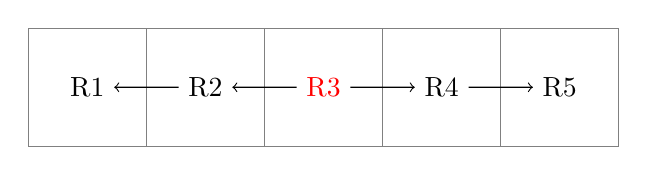
\begin{tikzpicture}[scale = 1.5]
\draw[color = gray] (0,0) grid[xstep = 1cm, ystep = 1cm] (5,1);
\node (R1) at (.5, .5) {R1};
\node (R2) at (1.5,.5) {R2};
\node (R3) [color =  red]  at (2.5,.5) {R3};
\node (R4) at (3.5,.5) {R4};
\node (R5) at (4.5,.5) {R5};
\draw [->] (R3) -- (R2);
\draw [->] (R3) -- (R4);
\draw [->] (R2) -- (R1);
\draw [->] (R4) -- (R5);
\end{tikzpicture}
\end{figure}

Similarly, if we study crime at the city level then somehow we should incorporate the possibility that crime is localized. For example identification of concentration or cluster of greater criminal activity has emerged as a central mechanism to targeting a criminal justice and crime prevention response to crime problem. These clusters of crime are commonly referred to as \textbf{hotpots}: geographic locations of high crime concentration, relative to the distribution of crime across the whole region of interest. 

Both examples implicitly state that geography location and distance matter. In fact, they reflect the importance of the first law of geography. According to Waldo Tobler: \emph{``everything is related to everything else'', but near things are more related than distant things}. This first law is the foundation of the fundamental concepts of \textbf{spatial dependence} and \textbf{spatial autocorrelation}.\index{Tobler's law}

%---------------------------------------------
\subsection{Spatial Dependence}\label{sec:spatial_dependence}\index{Spatial dependence}
%---------------------------------------------

Spatial dependence reflects a situation where values observed at one location or region, say observation $i$, depend on the values of neighboring observations at nearby locations. Formally, we might state

\begin{equation*}
  y_i = f(y_j),\quad i = 1,...,n\;, j\neq i.
\end{equation*}

In words, what happens in region $i$, depends on what happens in region $j$ for all $j\neq i$. Using our previous example, we would like to estimate 

\begin{equation*}
  \begin{aligned}
y_1 & = \beta_{21} y_2 + \beta_{31} y_3 + \beta_{41} y_4 + \beta_{51} y_5 + \epsilon_1 \\
y_2 & = \beta_{12} y_1 + \beta_{32} y_3 + \beta_{42} y_4 + \beta_{52} y_5 + \epsilon_2 \\
y_3 & = \beta_{13} y_1 + \beta_{23} y_2 + \beta_{43} y_4 + \beta_{53} y_5 + \epsilon_3 \\
y_4 & = \beta_{14} y_1 + \beta_{24} y_2 + \beta_{34} y_3 + \beta_{54} y_5 + \epsilon_4 \\
y_5 & = \beta_{15} y_1 + \beta_{25} y_2 + \beta_{35} y_3 + \beta_{45} y_5 + \epsilon_4 
\end{aligned}
\end{equation*}
%
where $\beta_{ji}$ is the effect of pollution of region $j$ on region $i$. However, it is easy to see that  this would be of little practical usefulness, since it would result in a system with many more parameters than observations: we have $n = 5$ observations, but 20 parameters to be estimated, which implies that we do not have sufficient degrees of freedom. Intuitively, once we allow for dependence relation between a set of $n$ observations/locations, there are potentially $n^2-n$ relations that could arise. We subtract $n$ from the potential $n^2$ dependence relations because we rule out dependence of an observation on itself. 

The key point is that, under standard econometric modeling, it is impossible to model spatial dependency. However, as we will see in the next sections, we might be able to incorporate spatial relationships more efficiently using the so-called spatial weight matrix. 

%===========================================
\subsection{Spatial Autocorrelation}\label{sec:Spatial_autocorrelation}
%===========================================

Another important concept is \textbf{spatial autocorrelation}\index{Spatial autocorrelation}. In space, the term autocorrelation refers to the correlation between the value of the variable at two different locations. Other ways of defining the same concept are: (1) correlation between the same attribute at two (or more) different locations, or (2) coincidence of values similarity with location similarity. Essentially, spatial autocorrelation is concerned with establishing whether the presence of a variable in one region in a regional system makes the presence of that variable in neighboring regions more, or less, likely.

The counterpart of spatial autocorrelation (and spatial dependency) is spatial randomness.  Spatial randomness means that we cannot observe any spatial pattern in the data. That is, the value we observe in some spatial unit is equally likely as in any other spatial unit. Spatial randomness is important because it will form the null hypothesis later. If rejected, then there is evidence of spatial structure.  

As an example, Figure \ref{fig:MR} plots the spatial distribution of poverty in the Metropolitan Region, Chile. It can be observed that there is some spatial pattern where communes with similar rate of poverty are clustered. 

\begin{figure}[ht]
  \caption{Spatial Distribution of Poverty in Metropolitan Region, Chile}
    \label{fig:MR}
    \centering
    	\begin{minipage}{.9\linewidth}
\begin{knitrout}
\definecolor{shadecolor}{rgb}{0.969, 0.969, 0.969}\color{fgcolor}

{\centering 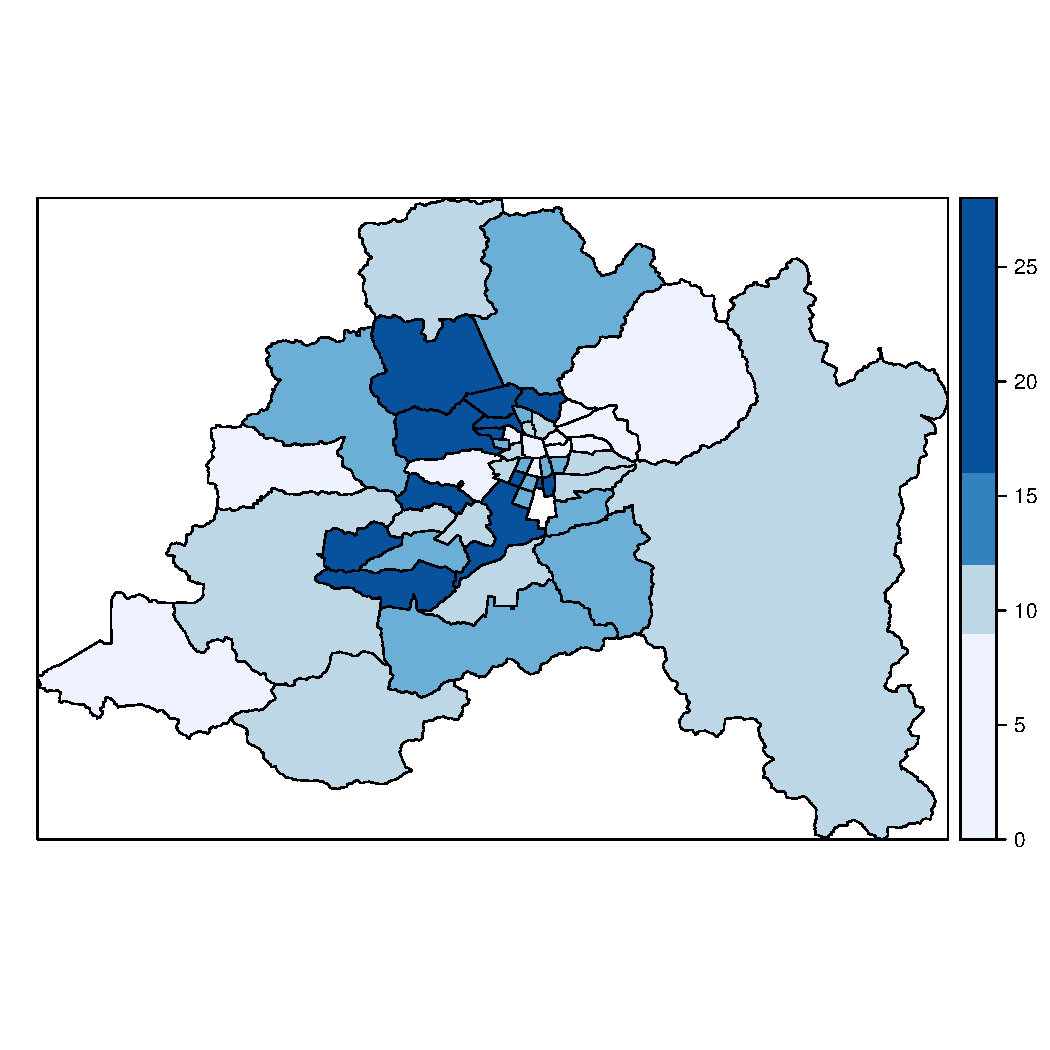
\includegraphics[width=8cm,height=8cm]{figure/MetroRegion-1} 

}


\end{knitrout}
\footnotesize
		\emph{Notes:} This graph shows the spatial distribution of poverty in the Metropolitan Region, Chile. 
	\end{minipage}	
\end{figure}

Formally, the existence of spatial autocorrelation may be expressed by the following moment conditions:

\begin{equation*}
  \cov(y_i, y_j) = \E(y_iy_j) - \E(y_i)\E(y_j)\neq 0\;\;\mbox{for}\;\; i \neq j,
\end{equation*}
%
where $y_i$ and $y_j$ are observations on a random variable at locations $i$ and $j$ in space, and $i,j$ can be points or areal units. Therefore, a nonzero spatial autocorrelation exists between attributes of a feature defined at locations $i$ and $j$ if the covariance between feature attribute values at those points is nonzero. If this covariance is \textbf{positive} (i.e., if data with attribute values above the mean tend to be near other data with values above the mean), then we say there is \textbf{positive spatial autocorrelation}; if the converse is true, then we say there is \textbf{negative spatial autocorrelation}. Figure \ref{fig:Autocorrelation} show an example of positive and negative spatial autocorrelation. 

\begin{figure}[ht]
  \caption{Spatial Autocorrelation}
    \label{fig:Autocorrelation}
    \centering
    	\begin{minipage}{1\linewidth}
\begin{knitrout}
\definecolor{shadecolor}{rgb}{0.969, 0.969, 0.969}\color{fgcolor}

{\centering 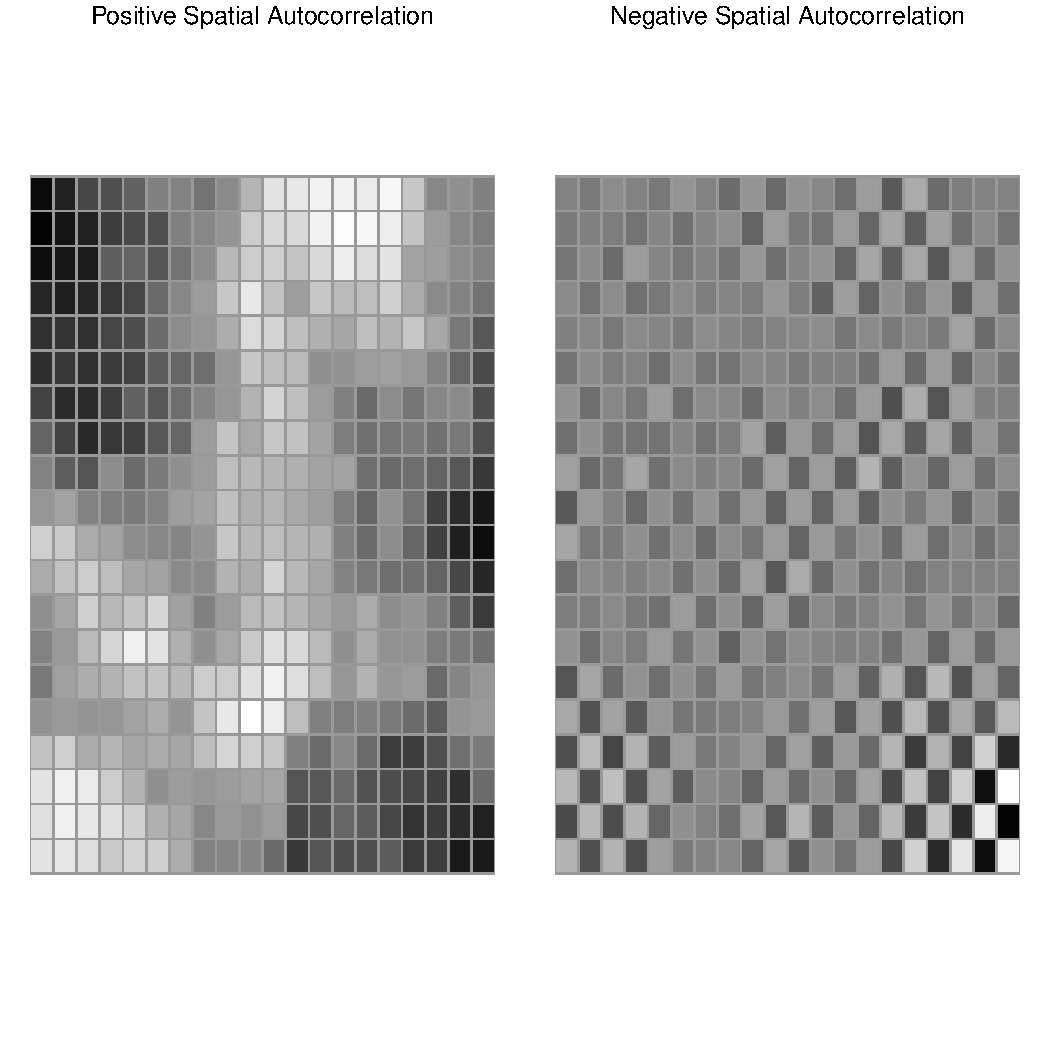
\includegraphics[width=10cm,height=10cm]{figure/Autocorrelation-1} 

}


\end{knitrout}
\footnotesize
		\emph{Notes:} Spatial Autocorrelation among 400 spatial units arranged in an 20-by-20 regular square lattice grid. Different gray-tones refer to different values of the variable ranging from low values (white) to high values (black). The left plot shows positive spatial autocorrelation, whereas right plot shows negative spatial autocorrelation. 
	\end{minipage}	
\end{figure}

Positive autocorrelation is much more common, but negative autocorrelation does exists, for example, in studies of welfare competition or federal grants competitions among local governments \citep{saavedra2000model, boarnet2002federal}, and studies of regional employment \citep{filiztekin2009regional, pavlyuk2011spatial}, the cross-border lottery shopping \citep{garrett2002revenue}, foreign direct investment in OECD countries \citep{garretsen2009fdi} and locations of Turkish manufacturing industry \citep{basdas2009spatial}. In short, we are interested in studying non-random spatial patterns and try to explain this non-randomness. Possible causes of non-randomness are \citep{gibbons2015spatial}:

\begin{enumerate}
	\item Economic agents may be randomly allocated across space but some characteristics of locations varies across space and influences outcomes. 
	\item Location may have no causal effect on outcomes, but outcomes may be correlated across space because heterogeneous individuals or firms are non-randomly allocated across space. 
	\item Individual or firms may be randomly allocated across  space but they interact so that decisions by one agent affects outcomes of other agents. 
	\item Individuals or firms may be non-randomly allocated across space and the characteristics of others nearby directly influences individual outcomes. 
\end{enumerate}


%********************************
\section{Spatial Weight Matrix}\index{Weight matrix}
%********************************

One of the crucial issues in spatial econometric is the problem of formally incorporating spatial dependence into the model. As we reviewed in Section~\ref{sec:spatial_dependence}, the main problem is that we have more parameter than observations. So, the question is: What would be a good criteria to define closeness in space? Or, in other words, how to determine which other units in the system influence the one under consideration?

The device typically used in spatial analysis to define the concept of closeness in space is the so-called ``spatial weight matrix'', or more simply, $\mW$ matrix. If we assume that there are $n$ spatial objects (regions, cities, countries), then $\mW$ will be a square matrix of dimension $n \times n$. This matrix imposes a structure in terms o what are the neighbors for each location. It assigns weights that measure the intensity of the relationship among pairs of spatial units. Thus, each element $(i,j)$ of $\mW$ -- which we denote by $w_{ij}$ -- expresses the degree of spatial proximity between the pair. This matrix can be represented in the form

\begin{equation*}
\mW = \begin{pmatrix}
        w_{11} & w_{12} & \hdots & w_{1n} \\ 
        w_{21} & w_{22} & \hdots & w_{2n} \\
        \vdots & \vdots & \ddots & \vdots \\
        w_{n1} & w_{n2} & \hdots & w_{nn} 
      \end{pmatrix}
\end{equation*}

Generally, we assume that the diagonal elements of this ``spatial neighbors'' matrix are set to zero: ``regions are not neighbors to themselves''.

A more formal definition of spatial weight matrix is the following:

\begin{definition}[Spatial Weight Matrix]\index{Weight matrix!Definition}\label{def:W}
  Let $n$ be the number of spatial units. The spatial weight matrix, $\mW$, a $n\times n$ \textbf{positive symmetric} and \textbf{non-stochastic} matrix with element $w_{ij}$ at location $i,j$. The values of $w_{ij}$ or the weights for each pair of locations are assigned by some preset rules which define the spatial relations among locations. By convention, $w_{ij} = 0$ for the diagonal elements.
\end{definition}

Positive symmetric means that $w_{ij}\geq 0$ and $w_{ij} = w_{ji}$, for $i\neq j$. Thus, the interactions between spatial units cannot be negative. Non-stochastic means that the researcher takes $\mW$ as known \emph{a priori}, and therefore, all results are conditional upon the specification of $\mW$.

The definition of $\mW$ also requires a rule for $w_{ij}$. In other words, we need to figure out how to assign a real number to $w_{ij}$, for $i\neq j$, representing the strength of the spatial relationship between $i$ and $j$. There are several ways of doing that. But, in general, there are two basic criteria. The first type establishes a relationship based on shared borders or vertices of lattice or irregular polygon data (contiguity). The second type establishes a relationship based on the distance between locations. Generally speaking, contiguity is most appropriate for geographic data expressed as polygons (so-called areal units), whereas distance is suited for point data, although in practice the distinction is not that absolute. 

%==========================================
\subsection{Weights Based on Boundaries}
%==========================================

The availability of polygon or lattice data permits the construction of contiguity-based spatial weight matrices. A typical specification of the contiguity relationship in the spatial weight matrix is

\begin{equation*}
  w_{ij}= 
   \begin{cases}
      1 & \mbox{if $i$ and $j$ are contiguous,} \\ 
      0 & \mbox{if $i$ and $j$ are not contiguous.} 
   \end{cases}
\end{equation*}

In a regular grid, neighbors (contiguity) can be defined in a number of ways. In analogy of the game of chess, rook contiguity, bishop contiguity and queen contiguity are distinguished.

\subsubsection{Rook Contiguity}\index{Weight matrix!Rook contiguity}

In this case, two locations are neighbors if they share at least part of a \textbf{common border or side}. In Figure~\ref{fig:Rook_cont_grid} we have a regular grid with 9 regions: each square represents a region. If for example we want to define the neighbors of region 5 using the rook criteria, then its neighbors will be regions 2, 4, 6 and 8. Those represent the regions filled in red. 

\begin{figure}[h]
\caption{Rook Contiguity}
\label{fig:Rook_cont_grid}
\centering
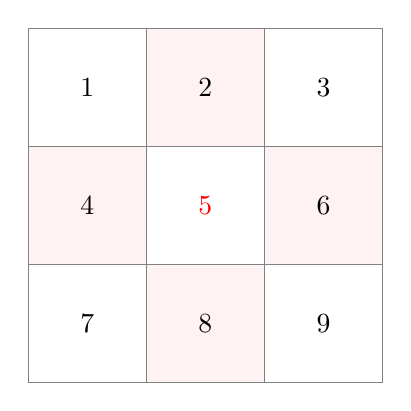
\begin{tikzpicture}[scale = 1.5]
\path [fill=red!5] (1,2) -- (2,2) -- (2,3) -- (1,3);
\path [fill=red!5] (1,0) -- (2,0) -- (2,1) -- (1,1);
\path [fill=red!5] (0,1) -- (1,1) -- (1,2) -- (0,2);
\path [fill=red!5] (2,1) -- (3,1) -- (3,2) -- (2,2);
\draw[color = gray] (0,0) grid[xstep = 1cm, ystep = 1cm] (3,3); % grid of 3 times 3
\node at (.5, 2.5) {1};
\node at (1.5, 2.5) {2};
\node at (2.5, 2.5) {3};
\node at (.5, 1.5) {4};
\node [color =  red] at (1.5,1.5) {5} ;
\node at (2.5,1.5) {6};
\node at (.5, .5) {7};
\node at (1.5,.5) {8};
\node at (2.5,.5) {9};
\end{tikzpicture}
\end{figure}

If we continue with this reasoning, then the $9\times 9$ $\mW$ matrix will be:

\begin{equation}
  \mW = 
  \begin{pmatrix}
     0 & 1 & 0 & 1 & 0 & 0 & 0 & 0 & 0 \\
     1 & 0 & 1 & 0 & 1 & 0 & 0 & 0 & 0 \\
     0 & 1 & 0 & 0 & 0 & 1 & 0 & 0 & 0 \\
     1 & 0 & 0 & 0 & 1 & 0 & 1 & 0 & 0 \\
     0 & 1 & 0 & 1 & 0 & 1 & 0 & 1 & 0 \\
     0 & 0 & 1 & 0 & 1 & 0 & 0 & 0 & 1 \\
     0 & 0 & 0 & 1 & 0 & 0 & 0 & 1 & 0 \\
     0 & 0 & 0 & 0 & 1 & 0 & 1 & 0 & 1 \\
     0 & 0 & 0 & 0 & 0 & 1 & 0 & 1 & 0 \\
  \end{pmatrix}
\end{equation}

\subsubsection{Bishop Contiguity}\index{Weight matrix!Bishop contiguity}

In bishop contiguity (\textbf{which is seldom used in practice}), region $i$'s neighbors are located at its corners. Figure~\ref{fig:Bishop_cont_grid} shows the neighbors of region 5 under this scheme. The neighbors are regions 1, 3, 7 and 9. Note that regions in the interior will have more neighbors than those in the periphery. 


\begin{figure}[h]
\caption{Bishop Contiguity}
\label{fig:Bishop_cont_grid}
\centering
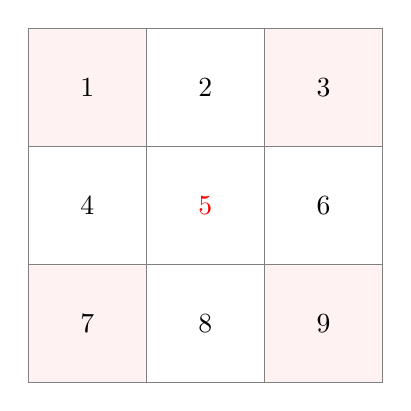
\begin{tikzpicture}[scale = 1.5]
\path [fill=red!5] (0,2) -- (1,2) -- (1,3) -- (0,3);
\path [fill=red!5] (0,0) -- (1,0) -- (1,1) -- (0,1);
\path [fill=red!5] (2,2) -- (3,2) -- (3,3) -- (2,3);
\path [fill=red!5] (2,0) -- (3,0) -- (3,1) -- (2,1);
\draw[color = gray] (0,0) grid[xstep = 1cm, ystep = 1cm] (3,3); % grid of 3 times 3
\node at (.5, 2.5) {1};
\node at (1.5, 2.5) {2};
\node at (2.5, 2.5) {3};
\node at (.5, 1.5) {4};
\node [color =  red] at (1.5,1.5) {5} ;
\node at (2.5,1.5) {6};
\node at (.5, .5) {7};
\node at (1.5,.5) {8};
\node at (2.5,.5) {9};
\end{tikzpicture}
\end{figure}

The resulting $\mW$ matrix will be:

\begin{equation*}
\mW = 
  \begin{pmatrix}
     0 & 0 & 0 & 0 & 1 & 0 & 0 & 0 & 0 \\
     0 & 0 & 0 & 1 & 0 & 1 & 0 & 0 & 0 \\
     0 & 0 & 0 & 0 & 1 & 0 & 0 & 0 & 0 \\
     0 & 1 & 0 & 0 & 0 & 0 & 0 & 1 & 0 \\
     1 & 0 & 1 & 0 & 0 & 0 & 1 & 0 & 1 \\
     0 & 1 & 0 & 0 & 0 & 0 & 0 & 1 & 0 \\
     0 & 0 & 0 & 0 & 1 & 0 & 0 & 0 & 0 \\
     0 & 0 & 0 & 1 & 0 & 1 & 0 & 0 & 0 \\
     0 & 0 & 0 & 0 & 1 & 0 & 0 & 0 & 0 \\
  \end{pmatrix}
\end{equation*}

This criteria is seldom used in practice. 

\subsubsection{Queen Contiguity}\index{Weight matrix!Queen contiguity}

In queen contiguity, any region that touches the boundary of region $i$, whether on a side or a single point, is considered neighbor. Under this criteria, the neighbors of 5 will be regions: 1, 2, 3, 4, 6, 7, 8 and 9.

\begin{figure}[h]
\caption{Queen Contiguity}
\label{fig:Queen_cont_grid}
\centering
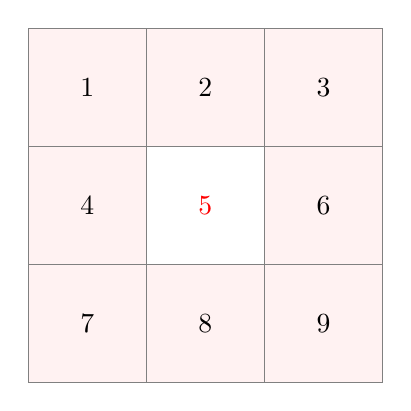
\begin{tikzpicture}[scale = 1.5]
\path [fill=red!5] (0,2) -- (1,2) -- (1,3) -- (0,3);
\path [fill=red!5] (0,0) -- (1,0) -- (1,1) -- (0,1);
\path [fill=red!5] (2,2) -- (3,2) -- (3,3) -- (2,3);
\path [fill=red!5] (2,0) -- (3,0) -- (3,1) -- (2,1);
\path [fill=red!5] (1,2) -- (2,2) -- (2,3) -- (1,3);
\path [fill=red!5] (1,0) -- (2,0) -- (2,1) -- (1,1);
\path [fill=red!5] (0,1) -- (1,1) -- (1,2) -- (0,2);
\path [fill=red!5] (2,1) -- (3,1) -- (3,2) -- (2,2);
\draw[color = gray] (0,0) grid[xstep = 1cm, ystep = 1cm] (3,3); % grid of 3 times 3
\node at (.5, 2.5) {1};
\node at (1.5, 2.5) {2};
\node at (2.5, 2.5) {3};
\node at (.5, 1.5) {4};
\node [color =  red] at (1.5,1.5) {5} ;
\node at (2.5,1.5) {6};
\node at (.5, .5) {7};
\node at (1.5,.5) {8};
\node at (2.5,.5) {9};
\end{tikzpicture}
\end{figure}


%=========================================
\subsection{Weights Based on Distance}\index{Weight matrix!Based on distance}
%=========================================

Weights may also be defined as a function of the distance between region $i$ and $j$, $d_{ij}$. This distance is usually computed as the distance between their centroids, but it may of course be between other relevant points for each spatial units, such as the capital -- or largest city-- or each region. Unlike the weights based on contiguity, matrices based on distances only need the coordinates of the points.

There are several ways of computing the distance between two spatial units. Let $x_i$ and $x_j$ be the longitude; and $y_i$ and $y_j$ the latitude coordinates for region $i$ and $j$, respectively. The most general concept of distance is the Minkowski metric:

\begin{equation*}
  d_{ij}^p = \left(\left|x_i - x_j\right|^p + \left|y_i - y_j\right|^p\right),
\end{equation*}
%
for two points $i$ and $j$, with respective coordinates $(x_i, y_i)$ and $(x_j, y_j)$, and with $p$ as the parameter. The most familiar special case is the Euclidean or straight line distance with $p = 2$:

\begin{equation*}
  d_{ij}^e = \sqrt{(x_i - x_j)^2 + (y_i - y_j)^2}.
\end{equation*}

Another employed metric is the Manhattan block distance. This measure only considers movement along the east-west and north-south directions, i.e., by straight angles. This yield a distance measure where $p = 1$:

\begin{equation*}
   d_{ij}^m = \left|x_i - x_j\right| + \left|y_i - y_j\right|.
\end{equation*}

All three measures presented above are useful if we consider the earth as a plane. For example, the Euclidean distance is the length of a straight line on a map, and is not necessarily the shortest distance if you take into account the curvature of the earth. The great circle distance take into account the curvature of Earth. Ships and aircraft usually follow the great circle geometry to minimize the distance and save time and money.  In particular, the great circle distance is computed as:

\begin{equation*}
d_{ij}^{cd} = r \times \arccos^{-1}\left[\cos|x_i - x_j| \cos y_i \cos y_j + \sin y_i \sin y_j \right]
\end{equation*}
%
where $r$ is the Earth's radius. The arc distance is obtained in miles with $r = 3959$ and in kilometers with $r = 6371$.

%=================================
\subsubsection{Inverse Distance}\label{sec:inverse_distance}
%=================================

Now we have to transform the information about the distances among spatial points into a weight scheme. The idea is that $w_{ijt}\to 0$ as $d_{ij}\to \infty$. In other words, the closer is $j$ to $i$, the larger $w_{ij}$ should be to conform to Tobler's first law. 

In the inverse distance weighting scheme, the weights are inversely related to separation distance as shown below:

\begin{equation*}
  w_{ij} =
  \begin{cases}
  \frac{1}{d_{ij}^{\alpha}} & \mbox{if} \;\;i \neq j \\
  0 & \mbox{if}\;\; i = j,
  \end{cases}
\end{equation*}
%
where the exponent $\alpha$ is a parameter that is usually set by the researcher. In practice, the parameters are seldom estimated, but typically set to $\alpha = 1$ or $\alpha = 2$. Therefore, the weights are given by  the reciprocal of the distance: the larger the distance between to spatial units, the lowest the spatial weight or the spatial connection. Finally, by convention, the diagonal elements of the spatial weights are set to zero and not computed. Plugging in a value of $d_{ii} = 0$ would yield division by zero for inverse distance weights. 

\subsubsection{Negative Exponential Model}

Here the weights decline exponentially with separation distance

\begin{equation*}
  w_{ij} = \exp\left(-\frac{d_{ij}}{\alpha}\right),
\end{equation*}
%
where $\alpha$ is a parameter that is commonly chosen by researcher. Since the weights are given by the exponential of the negative distance, the greater the distance between $i$ and $j$, the lower $w_{ij}$.

Both the inverse distance and the negative exponential distance depend not only on the parameter value and functional form, but also on the metric used for distance. Since the weights are inversely related to distance, larger values for the latter will yield small values for the former, and vice versa. This may be a problem in practice when the distances are so large that the corresponding inverse distance weights become close to zero, possible resulting in a zero spatial weight matrix. In addition, a potential problem may occur when the distance metric is such that distances take on values less than one, which is typically a not a desired result \citep{anselin2014modern}. 

\subsubsection{$k$-nearest Neighbors}

An alternative type of spatial weights that avoids the problem of isolates is to select the $k$-nearest neighbors. In contrast to the distance band, this is not a symmetric relation. However, a potential problem with this type of neighbors is the occurrence of ties, i.e., when more than one location $j$ has the same distance from $i$. A number of solutions exist to break the tie, from randomly selecting one the $k$-th order neighbors, to including all of them. 

\subsubsection{Threshold Distance (Distance Band Weights)}

In contrast to the $k$-nearest neighbors method, the threshold distance specifies that an region $i$ is neighbor of $j$ if the distance between them is less than a specified maximum distance:


\begin{equation*}
  w_{ij}= 
   \begin{cases}
      1 & \mbox{if}\;\; 0\leq d_{ij} \leq d_{max} \\ 
      0 & \mbox{if}\;\; d_{ij} > d_{max}.
   \end{cases}
\end{equation*}


To avoid isolates that would result from too stringent a critical distance, the distance must be chosen such that each location has at least one neighbor. Such a distance conforms to a max-min criterion, i.e., it is the largest of the nearest neighbor distances.

Finally, it is important to note that a weights matrix obtained from a distance band is always symmetric, since distance is a symmetric relation. 

%============================================
\subsection{Row-Standardized Weights Matrix}\index{Weight matrix!Row-standardization}
%============================================

In practice, the spatial weights are seldom used in their binary (or distance) form, but subject to a transformation or standardization. In particular, we would like to compute weighted averages in which more weight is placed on nearby observations than on distant observations. To do so, we can define a row-standardized weight matrix $\mW^s$, whose element $w_{ij}^s$ is given by:

\begin{equation*}
w_{ij}^s = \frac{w_{ij}}{\sum_j w_{ij}}.
\end{equation*}

This ensures that all weights are between 0 and 1 and facilities the interpretation of operation with the weights matrix as an averaging of neighboring values as we will see below. The row-standardized weights matrix also ensures that the spatial parameter in many spatial stochastic processes are comparable between models  \citep{AnselinBera1998}.

Another important feature is that, under row-standardization, the element of each row sum to unity and the sum of all weights, $S_0 = \sum_i\sum_j w_{ij} = n$, the total number of observations. This is a nice interpretation that we will explore later.

Another important issue is about symmetry. An important characteristic of symmetric matrix is that all its characteristics roots are real. However, \textbf{after the row standardization the matrices are no longer symmetric.} 

The row-standardized matrix is also known in the literature as the row-stochastic matrix:


\begin{definition}[Row-stochastic Matrix]
	A real $n\times n$ matrix $\mA$ is called \textbf{Markov} matrix, or \textbf{row-stochastic matrix} if 
		\begin{enumerate}
			\item $a_{ij} \geq 0$ for $1\leq i, j \leq n$;
			\item $\sum_{j=1}^n a_{ij} = 1$ for $1\leq i \leq n$
		\end{enumerate}
\end{definition}


An important characteristic of the row-stochastic matrix is related to its eigen values:


\begin{theorem}[Eigenvalues of row-stochastic Matrix]\label{teo:eigen_values}
	Every eigenvalue $\omega_i$ of a row-stochastic Matrix satisfies $\left|\vomega\right|\leq 1$
\end{theorem}

Therefore, the eigenvalues of the row-stochastic (i.e., row-normalized, row standardized or Markov) neighborhood matrix $\mW^s=(w_{ij}^s)$ are in the range $\left[-1, +1\right]$.

Finally, the behavior of $\mW^s$ is important for asymptotic properties of estimators and test statistics \citep[][pp. 244]{AnselinBera1998}. In particular, the $\mW$ matrix should be also exogenous, unless endogeneity is considered explicitly in the model specification. 

%============================================
\subsection{Spatial Lagged Variables}\label{sec:spatial_lag_var}\index{Weight matrix!Spatial lag}
%============================================

Now that we have discussed the spatial weight matrix, we can create the so-called \textbf{spatially lagged variables} or \textbf{spatial lag operator}. The spatial lag operator takes the form $\vy_L = \mW\vy$ with dimension $n \times 1$, where each element is given by $\vy_{Li} = \sum_{j}w_{ij}y_j$, i.e., a weighted average of the $\vy$ values in the neighbor of $i$.

For example:

\begin{equation*}
  \mW\vy =    \begin{pmatrix}
     0 & 1 & 0 \\
     1 & 0 & 1 \\
     0 & 1 & 0
  \end{pmatrix}
  \begin{pmatrix}
     10 \\
     50 \\
     30
  \end{pmatrix} =
  \begin{pmatrix}
     50 \\
     10 + 30 \\
     50
  \end{pmatrix}.
\end{equation*}

Using a row-standardized weight matrix:

\begin{equation*}
  \mW\vy =    \begin{pmatrix}
     0 & 1 & 0 \\
     0.5 & 0 & 0.5 \\
     0 & 1 & 0
  \end{pmatrix}
  \begin{pmatrix}
     10 \\
     50 \\
     30
  \end{pmatrix} =
  \begin{pmatrix}
     50 \\
     5 + 15 \\
     50
  \end{pmatrix}.
\end{equation*}

As a result, for spatial unit $i$, the spatial lag of $y_i$, referred as $\vy_{Li}$ ( the variable $Wy$ observed for location $i$) is:

\begin{equation*}
  \vy_{Li} = w_{i, 1}y_i + w_{i, 2}y_2 + ... + w_{i, n}y_n, 
\end{equation*}
%
or,

\begin{equation*}
  \vy_{Li} = \sum_{j = 1}^nw_{i,j}y_j,
\end{equation*}
%
where the weights $w_{ij}$ consists of the elements of the $i$th row of the matrix $\mW$, matched up with the corresponding elements of the vector $\vy$. In other words, this is a weighted sum of the values observed at neighboring locations, since the non-neighbors are not included. 

\begin{remark}
As stated by \citet[][p. 23-24]{anselin1988spatial}, standardization must be done with caution.\footnote{See also \citet[][p. 12]{elhorst2014spatial} and references therein.} For example, when the weights are based on an inverse distance function (or similar concept of distance decay), which has a meaningful economic interpretation, scaling the rows so that the weights sum to one may result in a loss of that interpretation. Can you give an example?
\end{remark}


%============================================
\subsection{Higher Order Spatial}\label{sec:HSO}\index{Weight matrix!Higher order}
%============================================

So far we have learned how to define the geographical space by matrix $\mW$. However, an interesting question is how to define higher-order neighbors. For example, we may be interested in defining the neighbors of the neighbors of a spatial unit. Or even we might be interested in the neighbors of neighbors of neighbors of spatial unit $i$. To discuss this interesting case we need to define \textbf{higher-order spatial weight matrices}. 

We define the higher-order spatial weight matrix $l$ as $\mW^l$. So, for example the spatial weight of order $l=2$ is given by $\mW^2 = \mW\mW$, spatial weight matrix of order $l = 3$ is given by $\mW^3 = \mW\mW\mW$, and so on. What is the meaning of the element $w_{ij}$ in this case? For spatial weights of order 2, the element $w_{ij}$ of the weight matrix is 1 if polygon $j$ is adjacent to the first order neighbors of polygon $i$ and is 0 otherwise. Thus, for spatial neighbor weights of order $n$, the element $w_{ij}$ of the weight matrix $\mW$ is 1 if polygon $j$ is adjacent to the neighbors of order $n-1$ of polygon $i$, and is 0 otherwise. 

To illustrate these points, consider the following spatial structure for our example in Section \ref{sec:why_se}:

\begin{equation}\label{eq:W5x5}
\mW = \begin{pmatrix}
      0 & 1 & 0 & 0 & 0 \\
      1 & 0 & 1 & 0 & 0 \\
      0 & 1 & 0 & 1 & 0 \\
      0 & 0 & 1 & 0 & 1 \\
      0 & 0 & 0 & 1 & 0
      \end{pmatrix}.
\end{equation}

Then $\mW^2 = \mW\mW$ based on the $5\times 5$ first-order contiguity matrix $\mW$ from (\ref{eq:W5x5}) is:

\begin{equation}
\mW^2 = \begin{pmatrix}\label{eq:W25x5}
      1 & 0 & 1 & 0 & 0 \\
      0 & 2 & 0 & 1 & 0 \\
      1 & 0 & 2 & 0 & 1 \\
      0 & 1 & 0 & 2 & 0 \\
      0 & 0 & 1 & 0 & 1
      \end{pmatrix}
\end{equation}

Note that for region $R1$, the second-order neighbors are regions $R1$ and $R3$. That is, region $R1$ is a second-order neighbor to itself as well as to region $R3$, which is a neighbor to the neighboring region $R2$. 

Now consider R2. The first panel of Figure \ref{fig:example_hon} shows the first-order neighbors of $R2$ given by the spatial weight matrix in (\ref{eq:W5x5}): the first-order neighbors are R1 and R3. Panel B considers the second-order neighbors of $R2$: the second-order neighbors are $R2$ itself and $R4$. To understand this, note that there is a feedback effect from the first impact from $R2$ coming from $R1$ and $R3$ (first-order neighbors of $R2$). This explains why the element $w^2_{22} = 2$. Moreover, there is an indirect effect coming from $R4$ through $R3$ that finally impacts $R2$.  This represents the value of 1 for the element $w^2_{24}$.

Similarly, for region $R3$, the second-order neighbors are regions $R1$ (which is a neighbor to the neighboring region $R2$), $R3$ (a second-order neighbor to itself), and $R5$ (which is a neighbor to the neighboring region $R4$). 

\begin{figure}[ht]
\caption{Higher-Order Neighbors}
\label{fig:example_hon}
\centering
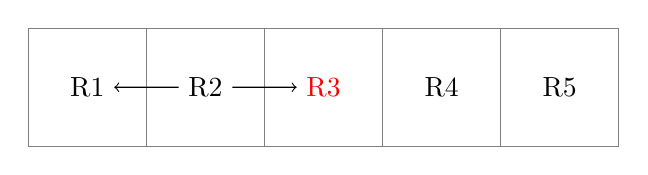
\begin{tikzpicture}[scale = 1.5]
\draw[color = gray] (0,0) grid[xstep = 1cm, ystep = 1cm] (5,1);
\node (R1) at (.5, .5) {R1};
\node (R2) at (1.5,.5) {R2};
\node (R3) [color =  red]  at (2.5,.5) {R3};
\node (R4) at (3.5,.5) {R4};
\node (R5) at (4.5,.5) {R5};
\draw [->] (R2) -- (R1);
\draw [->] (R2) -- (R3);
\end{tikzpicture}
\\
\vspace{1cm}
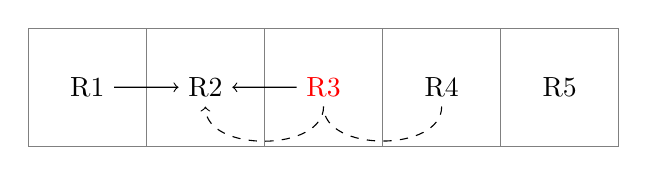
\begin{tikzpicture}[scale = 1.5]
\draw[color = gray] (0,0) grid[xstep = 1cm, ystep = 1cm] (5,1);
\node (R1) at (.5, .5) {R1};
\node (R2) at (1.5,.5) {R2};
\node (R3) [color =  red]  at (2.5,.5) {R3};
\node (R4) at (3.5,.5) {R4};
\node (R5) at (4.5,.5) {R5};
\draw [->] (R1) -- (R2);
\draw [->] (R3) -- (R2);
\draw [->, dashed] (R4) to[out= 270,in=270] (R3) to[out=270,in=270] (R2);
\end{tikzpicture}
\end{figure}

Similarly, the third-order neighbors are: 


\begin{equation*}
\mW^3 = \begin{pmatrix}
      0 & 2 & 0 & 1 & 0 \\
      2 & 0 & 3 & 0 & 1 \\
      0 & 3 & 0 & 3 & 0 \\
      1 & 0 & 3 & 0 & 2 \\
      0 & 1 & 0 & 2 & 1
      \end{pmatrix}
\end{equation*}

Could you explain the elements of this matrix?


%============================================
\section{Examples of Weight Matrices in R}
%============================================

Creating spatial weight matrices by hand is tedious (and in some cases almost impossible). However, there exists several statistical software that allow us to create them in a very simply fashion.  First, we need the \textbf{shape file}, which has geographical information.  The shapefile format is a digital vector storage for storing geometric location and associated attribute information. Nowadays it is possible to read and write geographical datasets using the shapefile format with a wide variety of software.

The shapefile format is simple because it can store the primate geometric data types of points, lines and polygons. Shapes (points/lines/polygons) together with data attributes can create infinitely many representations about geographic data. The three mandatory files have filename extensions \texttt{.shp, .shx}, and \texttt{.dbf}. The actual shapefile relates specifically to the \texttt{.shp} file, but alone is incomplete for distribution as the other supporting files are required. The characteristics of each file is the following:

\begin{itemize}
  \item \texttt{.shp}: shape format; the feature geometry itself,
  \item \texttt{.shx}: shape index format; a positional index of the feature geometry to allow seeking forwards and backwards quickly,
  \item \texttt{.dbf}: attribute format; columnar attributes for each shape, in \texttt{dBase} IV format. 
\end{itemize}

For simplicity in showing how to create neighbor objects in \proglang{R}, we work on the map consisting of the communes of the Metropolitan Region in Chile. 

We first need to load the Metropolitan Region shape file in \proglang{R}. To do so, we will use the \pkg{sf} package, which allows us reading and handling spatial objects. 

\begin{knitrout}
\definecolor{shadecolor}{rgb}{0.969, 0.969, 0.969}\color{fgcolor}\begin{kframe}
\begin{alltt}
\hlcom{#Load package}
\hlkwd{library}\hlstd{(}\hlstr{"sf"}\hlstd{)}
\end{alltt}
\end{kframe}
\end{knitrout}

If the shape file \code{mr\_chile.shp} is in the same working directory, then we can load it into \proglang{R} using the command \code{read\_sf}:

\begin{knitrout}
\definecolor{shadecolor}{rgb}{0.969, 0.969, 0.969}\color{fgcolor}\begin{kframe}
\begin{alltt}
\hlcom{# Read shape file}
\hlstd{mr} \hlkwb{<-} \hlkwd{read_sf}\hlstd{(}\hlstr{"mr_chile.shp"}\hlstd{)}
\hlkwd{class}\hlstd{(mr)}
\end{alltt}
\begin{verbatim}
## [1] "sf"         "tbl_df"     "tbl"        "data.frame"
\end{verbatim}
\end{kframe}
\end{knitrout}

The function \code{read\_sf} reads data from the shapefile into a \code{Spatial} object of class ``\code{sf}''. The function \code{names} give us the name of the variables in the \texttt{.dbf} file associated with the shape file. 

\begin{knitrout}
\definecolor{shadecolor}{rgb}{0.969, 0.969, 0.969}\color{fgcolor}\begin{kframe}
\begin{alltt}
\hlcom{# Names of the variables in .dbf}
\hlkwd{names}\hlstd{(mr)}
\end{alltt}
\begin{verbatim}
##  [1] "ID"         "NAME"       "NAME2"      "URB_POP"    "RUR_POP"   
##  [6] "MALE_POP"   "TOT_POP"    "FEM_POP"    "N_PARKS"    "N_PLAZA"   
## [11] "CONS_HOUSE" "M2_CONS_HA" "GREEN_AREA" "AREA"       "POVERTY"   
## [16] "PER_CONTR_" "PER_HON_SA" "PER_PLANT_" "NURSES"     "DOCTORS"   
## [21] "CONSULT_RU" "CONSULT_UR" "POSTAS"     "ESTAB_MUN_" "PSU_MUN_PR"
## [26] "PSU_PART_P" "PSU_SUB_PR" "STUDENT_SU" "STUDENT_PA" "STUDENT_MU"
## [31] "geometry"
\end{verbatim}
\end{kframe}
\end{knitrout}

We can plot the shapefile using the generic function \code{plot} in the following way

\begin{knitrout}
\definecolor{shadecolor}{rgb}{0.969, 0.969, 0.969}\color{fgcolor}\begin{kframe}
\begin{alltt}
\hlcom{# Plot shapefile}
\hlkwd{plot}\hlstd{(}\hlkwd{st_geometry}\hlstd{(mr),} \hlkwc{main} \hlstd{=} \hlstr{"Metropolitan Region-Chile"}\hlstd{,} \hlkwc{axes} \hlstd{=} \hlnum{TRUE}\hlstd{)}
\end{alltt}
\end{kframe}
\end{knitrout}

The metropolitan region with the 52 communes is shown in Figure \ref{fig:plot_mr}.

\begin{figure}[h]
  \caption{Plotting a Map in R}
    \label{fig:plot_mr}
\begin{knitrout}
\definecolor{shadecolor}{rgb}{0.969, 0.969, 0.969}\color{fgcolor}

{\centering 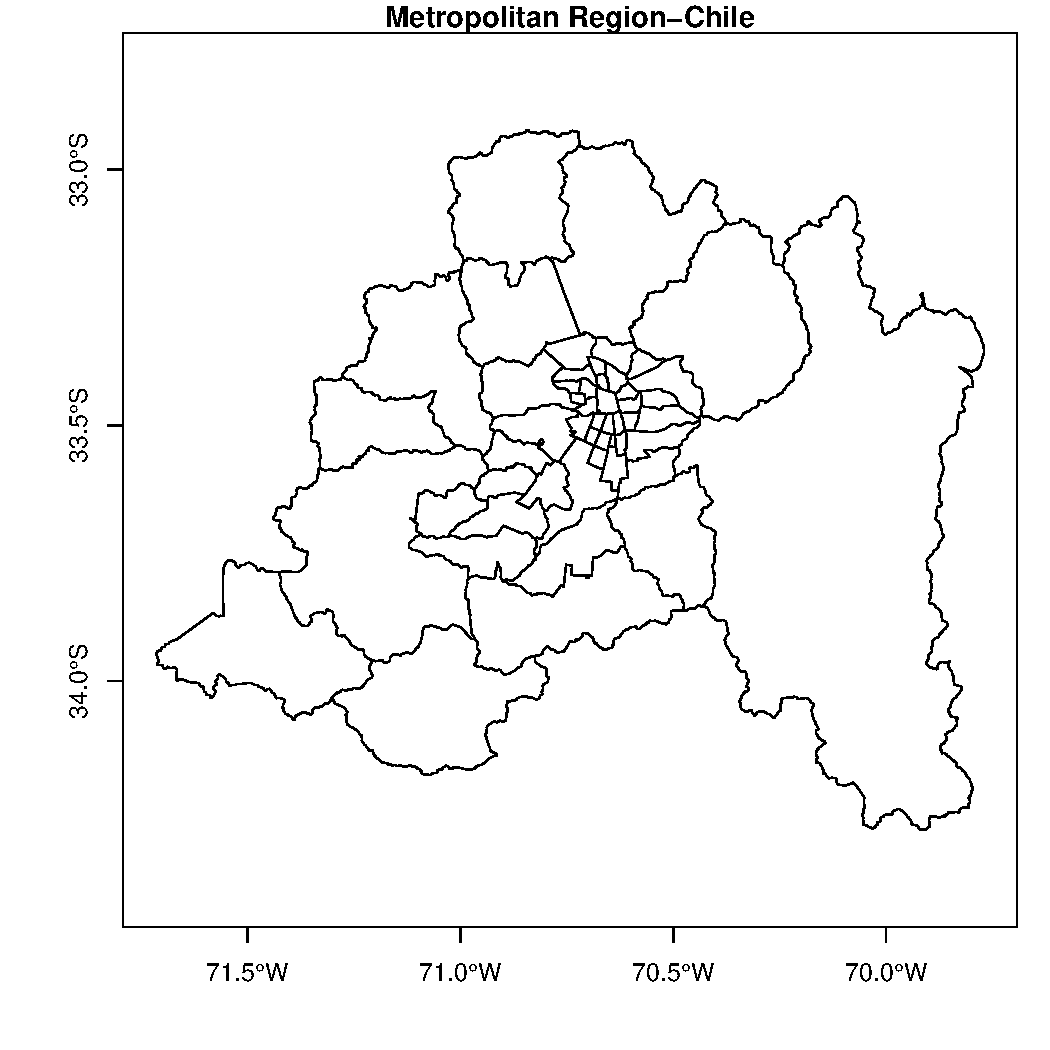
\includegraphics[width=8cm,height=8cm]{figure/plot_mr-1} 

}


\end{knitrout}
\end{figure}

%===============================================
\subsection{Creating Contiguity Neighbors}
%===============================================

To create spatial weight matrices we need the \pkg{spdep} package \citep{bivand2013computing}. After installing it, we load the package

\begin{knitrout}
\definecolor{shadecolor}{rgb}{0.969, 0.969, 0.969}\color{fgcolor}\begin{kframe}
\begin{alltt}
\hlcom{#Load package}
\hlkwd{library}\hlstd{(}\hlstr{"spdep"}\hlstd{)}
\end{alltt}
\end{kframe}
\end{knitrout}

In the \pkg{spdep} package, neighbor relationships between $n$ observations are represented by an object of class ``\code{nb}''. This object is a list of length $n$ with the index numbers of neighbors of each component recorded as an integer vector. If any observation has no neighbors, the component contains an integer zero. 


The function \code{poly2nb} is used in order to construct weight matrices based on \textbf{contiguity}. Specifically, it creates a ``neighbors list'' based on regions with contiguous boundaries of class ``\code{nb}''. Check out \code{help(polynb)} to see all the details and options. 

First, we create a neighbor list based on the `Queen' criteria for the communes of the Metropolitan Region\index{Weight matrix!poly2nb function}:

\begin{knitrout}
\definecolor{shadecolor}{rgb}{0.969, 0.969, 0.969}\color{fgcolor}\begin{kframe}
\begin{alltt}
\hlcom{# Create queen W}
\hlkwd{sf_use_s2}\hlstd{(}\hlnum{FALSE}\hlstd{)}
\hlstd{queen.w} \hlkwb{<-} \hlkwd{poly2nb}\hlstd{(}\hlkwd{as}\hlstd{(mr,} \hlstr{"Spatial"}\hlstd{),} \hlkwc{queen} \hlstd{=}  \hlnum{TRUE}\hlstd{,} \hlkwc{row.names} \hlstd{= mr}\hlopt{$}\hlstd{NAME)}
\end{alltt}
\end{kframe}
\end{knitrout}

Since we have an \code{nb} object to examine, we can present the standard methods for these objects. There are \code{print}, \code{summary}, \code{plot}, and other methods. The characteristics of the weights are obtained with the usual \code{summary} command:

\begin{knitrout}
\definecolor{shadecolor}{rgb}{0.969, 0.969, 0.969}\color{fgcolor}\begin{kframe}
\begin{alltt}
\hlcom{# Summary of W}
\hlkwd{summary}\hlstd{(queen.w)}
\end{alltt}
\begin{verbatim}
## Neighbour list object:
## Number of regions: 52 
## Number of nonzero links: 292 
## Percentage nonzero weights: 10.79882 
## Average number of links: 5.615385 
## Link number distribution:
## 
##  2  3  4  5  6  7  8  9 10 12 
##  3  2  7 15 10 10  2  1  1  1 
## 3 least connected regions:
## Tiltil San Pedro Maria Pinto with 2 links
## 1 most connected region:
## San Bernardo with 12 links
\end{verbatim}
\end{kframe}
\end{knitrout}

The output presents important information about the neighbors: it shows the number of regions, which corresponds to 52 in this example; the number of nonzero links; the percentage of nonzero weights; the average number of links, and so on. 

The commune of San Bernardo is most connected region with 12 neighbors under the queen scheme. The least connected regions are Tiltil, San Pedro, and Maria Pinto with 2 neighbors each of them. The output also shows the distribution of neighbors.  For example, 7 out of 52 regions has 4 neighbors and only 2 communes has 8 neighbors.  

To transform the \code{list} into an actual matrix $\mW$, we can use the function \code{nb2listw}\index{Weight matrix!nb2listw function}:


\begin{knitrout}
\definecolor{shadecolor}{rgb}{0.969, 0.969, 0.969}\color{fgcolor}\begin{kframe}
\begin{alltt}
\hlcom{# From list to matrix}
\hlstd{queen.wl} \hlkwb{<-} \hlkwd{nb2listw}\hlstd{(queen.w,} \hlkwc{style} \hlstd{=} \hlstr{"W"}\hlstd{)}
\hlkwd{summary}\hlstd{(queen.wl)}
\end{alltt}
\begin{verbatim}
## Characteristics of weights list object:
## Neighbour list object:
## Number of regions: 52 
## Number of nonzero links: 292 
## Percentage nonzero weights: 10.79882 
## Average number of links: 5.615385 
## Link number distribution:
## 
##  2  3  4  5  6  7  8  9 10 12 
##  3  2  7 15 10 10  2  1  1  1 
## 3 least connected regions:
## Tiltil San Pedro Maria Pinto with 2 links
## 1 most connected region:
## San Bernardo with 12 links
## 
## Weights style: W 
## Weights constants summary:
##    n   nn S0       S1      S2
## W 52 2704 52 19.76751 216.466
\end{verbatim}
\end{kframe}
\end{knitrout}

An important argument of the function is \code{style}. This argument indicates what type of matrix to create. For example, \code{style = "W"} creates a row-standardize matrix so that $w^s_{ij} = w_{ij}/ \sum_j w_{ij}$. After normalization, each row of $\mW^s$ will sum to 1. \code{"B"} is the basic binary coding; and \code{"C"} is globally standardize, that is, $w^s_{ij} = w_{ij} \cdot (n/ \sum_{i}\sum_j w_{ij})$. If \code{style = "U"}, then $w^s_{ij} = w_{ij}/ \sum_i\sum_j w_{ij}$. In a \code{minmax} matrix, the $(i,j)$th element of $\mW^s$  becomes $w^s_{ij} = w_{ij} / \min\left\lbrace \max_i(\tau_i), \max_i(c_i)\right\rbrace$, with $\max_i(\tau_i)$ being the largest row sum of $\mW$ and $\max_i(c_i)$ being the largest column sum of $\mW$ \citep{kelejian2010specification}. Finally, \code{"S"} is the variance-stabilizing coding scheme where $w^s_{ij} = w_{ij}/ \sqrt{\sum_j w_{ij} ^2}$ \citep{tiefelsdorf1999variance}. 

Furthermore, the \code{summary} function reports constants used in the inference for global spatial autocorrelation statistics, which we will discuss later. 

We can also see the attributes of the object using the function \code{attributes}:


\begin{knitrout}
\definecolor{shadecolor}{rgb}{0.969, 0.969, 0.969}\color{fgcolor}\begin{kframe}
\begin{alltt}
\hlcom{# Attributes of wlist}
\hlkwd{attributes}\hlstd{(queen.w)}
\end{alltt}
\begin{verbatim}
## $class
## [1] "nb"
## 
## $region.id
##  [1] "Santiago"            "Cerillos"            "Cerro Navia"        
##  [4] "Conchali"            "El Bosque"           "Estacion Central"   
##  [7] "La Cisterna"         "La Florida"          "La Granja"          
## [10] "La Pintana"          "La Reina"            "Lo Espejo"          
## [13] "Lo Prado"            "Macul"               "Nunoa"              
## [16] "Pedro Aguirre Cerda" "Penalolen"           "Providencia"        
## [19] "Quinta Normal"       "Recoleta"            "Renca"              
## [22] "San Joaquin"         "San Miguel"          "San Ramon"          
## [25] "Independencia"       "Puente Alto"         "Las Condes"         
## [28] "Vitacura"            "Quilicura"           "Huechuraba"         
## [31] "Maipu"               "Pudahuel"            "San Bernardo"       
## [34] "Tiltil"              "Lampa"               "Colina"             
## [37] "Lo Barnechea"        "Pirque"              "Paine"              
## [40] "Buin"                "Alhue"               "Melipilla"          
## [43] "San Pedro"           "Maria Pinto"         "Curacavi"           
## [46] "Penaflor"            "Calera de Tango"     "Padre Hurtado"      
## [49] "El Monte"            "Talagante"           "Isla de Maipo"      
## [52] "San Jose de Maipo"  
## 
## $call
## poly2nb(pl = as(mr, "Spatial"), row.names = mr$NAME, queen = TRUE)
## 
## $type
## [1] "queen"
## 
## $sym
## [1] TRUE
\end{verbatim}
\end{kframe}
\end{knitrout}

We may ask whether the matrix is symmetric using:

\begin{knitrout}
\definecolor{shadecolor}{rgb}{0.969, 0.969, 0.969}\color{fgcolor}\begin{kframe}
\begin{alltt}
\hlcom{# Symmetric W}
\hlkwd{is.symmetric.nb}\hlstd{(queen.w)}
\end{alltt}
\begin{verbatim}
## [1] TRUE
\end{verbatim}
\end{kframe}
\end{knitrout}

As we previously discussed, generally weight matrix based on boundaries are symmetric. Now, we construct a binary matrix using the Rook criteria:

\begin{knitrout}
\definecolor{shadecolor}{rgb}{0.969, 0.969, 0.969}\color{fgcolor}\begin{kframe}
\begin{alltt}
\hlcom{# Rook W}
\hlstd{rook.w} \hlkwb{<-} \hlkwd{poly2nb}\hlstd{(}\hlkwd{as}\hlstd{(mr,} \hlstr{"Spatial"}\hlstd{),} \hlkwc{row.names} \hlstd{= mr}\hlopt{$}\hlstd{NAME,} \hlkwc{queen} \hlstd{=}  \hlnum{FALSE}\hlstd{)}
\hlkwd{summary}\hlstd{(rook.w)}
\end{alltt}
\begin{verbatim}
## Neighbour list object:
## Number of regions: 52 
## Number of nonzero links: 272 
## Percentage nonzero weights: 10.05917 
## Average number of links: 5.230769 
## Link number distribution:
## 
##  2  3  4  5  6  7  8  9 10 
##  3  3 12 16  7  6  2  1  2 
## 3 least connected regions:
## Tiltil San Pedro Maria Pinto with 2 links
## 2 most connected regions:
## Santiago San Bernardo with 10 links
\end{verbatim}
\end{kframe}
\end{knitrout}

Finally, we can plot the weight matrices using the following set of commands (see Figure \ref{fig:Queen-Rook}). 

\begin{knitrout}
\definecolor{shadecolor}{rgb}{0.969, 0.969, 0.969}\color{fgcolor}\begin{kframe}
\begin{alltt}
\hlcom{# Plot Queen and Rook W Matrices}
\hlkwd{plot}\hlstd{(}\hlkwd{st_geometry}\hlstd{(mr),} \hlkwc{border} \hlstd{=} \hlstr{"grey"}\hlstd{)}
\hlstd{coords} \hlkwb{<-} \hlkwd{st_coordinates}\hlstd{(}\hlkwd{st_centroid}\hlstd{(}\hlkwd{st_geometry}\hlstd{(mr)))}
\hlkwd{plot}\hlstd{(queen.w, coords,} \hlkwc{add} \hlstd{=}  \hlnum{TRUE}\hlstd{,} \hlkwc{col} \hlstd{=} \hlstr{"red"}\hlstd{)}
\hlkwd{plot}\hlstd{(rook.w, coords,} \hlkwc{add} \hlstd{=}  \hlnum{TRUE}\hlstd{,} \hlkwc{col} \hlstd{=} \hlstr{"yellow"}\hlstd{)}
\end{alltt}
\end{kframe}
\end{knitrout}

\begin{figure}
  \caption{Queen and Rook Criteria for MR}
    \label{fig:Queen-Rook}
\begin{knitrout}
\definecolor{shadecolor}{rgb}{0.969, 0.969, 0.969}\color{fgcolor}

{\centering 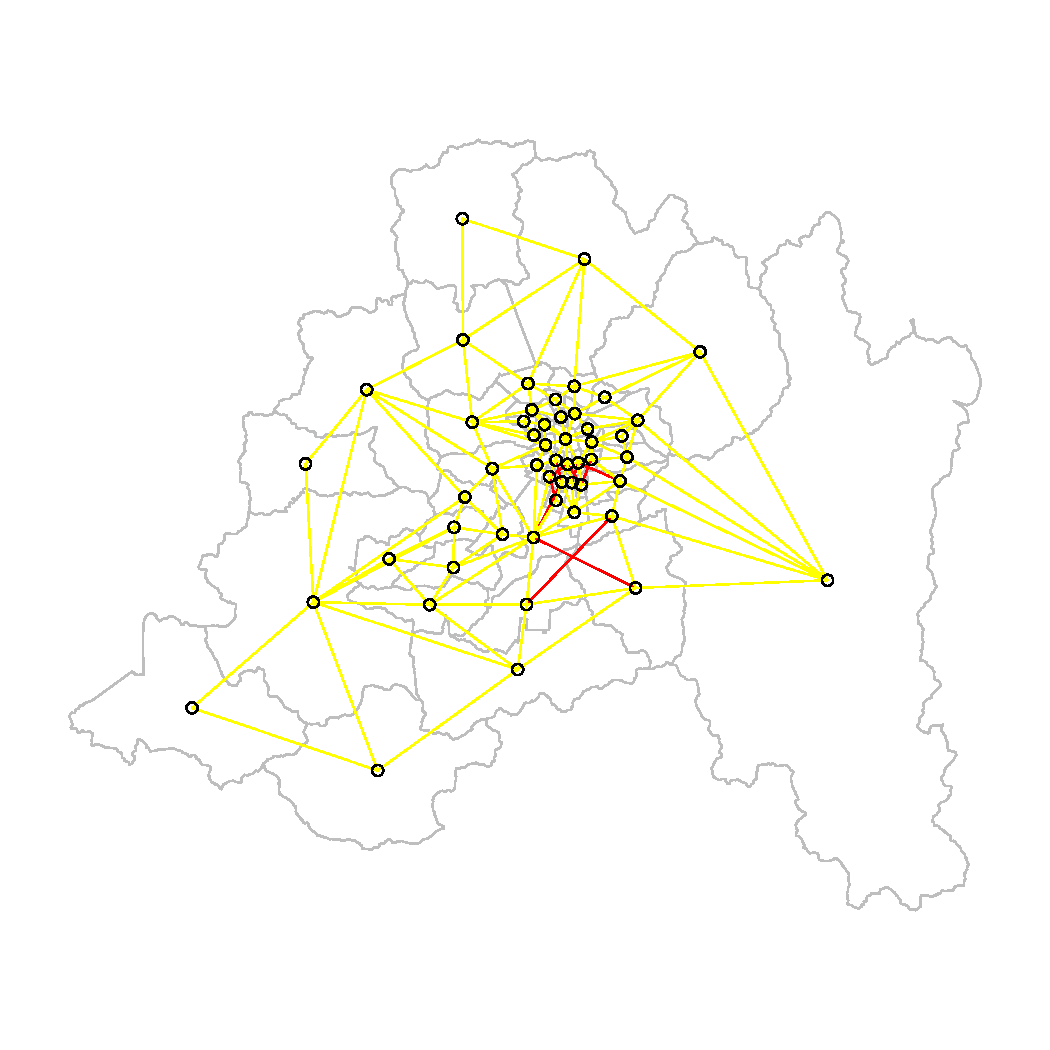
\includegraphics[width=8cm,height=8cm]{figure/plot-queen-rookT-1} 

}


\end{knitrout}
\end{figure}

%==================================================
\subsection{Creating Distance-based Neighbors}
%==================================================

We now construct spatial weight matrices using the $k$-nearest neighbors criteria\index{Weight matrix!knearneigh function}. 

\begin{knitrout}
\definecolor{shadecolor}{rgb}{0.969, 0.969, 0.969}\color{fgcolor}\begin{kframe}
\begin{alltt}
\hlcom{# K-neighbors}
\hlkwd{head}\hlstd{(coords,} \hlnum{5}\hlstd{)}                                       \hlcom{# show coordinates}
\end{alltt}
\begin{verbatim}
##           X         Y
## 1 -70.65599 -33.45406
## 2 -70.71742 -33.50027
## 3 -70.74504 -33.42278
## 4 -70.67735 -33.38372
## 5 -70.67640 -33.56294
\end{verbatim}
\begin{alltt}
\hlstd{k1neigh} \hlkwb{<-} \hlkwd{knearneigh}\hlstd{(coords,} \hlkwc{k} \hlstd{=} \hlnum{1}\hlstd{,} \hlkwc{longlat} \hlstd{=} \hlnum{TRUE}\hlstd{)}  \hlcom{# 1-nearest neighbor}
\hlstd{k2neigh} \hlkwb{<-} \hlkwd{knearneigh}\hlstd{(coords,} \hlkwc{k} \hlstd{=} \hlnum{2}\hlstd{,} \hlkwc{longlat} \hlstd{=} \hlnum{TRUE}\hlstd{)}  \hlcom{# 2-nearest neighbor}
\end{alltt}
\end{kframe}
\end{knitrout}

The function \code{coords} extract the spatial coordinates from the shape file, whereas the function \code{knearneigh} returns a matrix with the indices of points belonging to the set of the $k$-nearest neighbors of each other. The argument \code{k} indicates the number of nearest neighbors to be returned. If point coordinates are longitude-latitude decimal degrees, then distances are measured in kilometers if \code{longlat = TRUE}. Furthermore, if \code{longlat = TRUE}, great circle distances are used. Note that the objects \code{k1neigh} and \code{k2neigh} are of class \code{knn}.

Weight matrices based on inverse distance can be computed in the following way (see Section \ref{sec:inverse_distance}):

\begin{knitrout}
\definecolor{shadecolor}{rgb}{0.969, 0.969, 0.969}\color{fgcolor}\begin{kframe}
\begin{alltt}
\hlcom{# Inverse weight matrix}
\hlstd{dist.mat} \hlkwb{<-} \hlkwd{as.matrix}\hlstd{(}\hlkwd{dist}\hlstd{(coords,} \hlkwc{method} \hlstd{=} \hlstr{"euclidean"}\hlstd{))}
\hlstd{dist.mat[}\hlnum{1}\hlopt{:}\hlnum{5}\hlstd{,} \hlnum{1}\hlopt{:}\hlnum{5}\hlstd{]}
\end{alltt}
\begin{verbatim}
##            1          2          3          4          5
## 1 0.00000000 0.07687010 0.09438408 0.07350782 0.11078109
## 2 0.07687010 0.00000000 0.08226867 0.12324109 0.07489489
## 3 0.09438408 0.08226867 0.00000000 0.07814455 0.15606360
## 4 0.07350782 0.12324109 0.07814455 0.00000000 0.17922003
## 5 0.11078109 0.07489489 0.15606360 0.17922003 0.00000000
\end{verbatim}
\begin{alltt}
\hlstd{dist.mat.inv} \hlkwb{<-} \hlnum{1} \hlopt{/} \hlstd{dist.mat} \hlcom{# 1 / d_\{ij\}}
\hlkwd{diag}\hlstd{(dist.mat.inv)} \hlkwb{<-} \hlnum{0}      \hlcom{# 0 in the diagonal}
\hlstd{dist.mat.inv[}\hlnum{1}\hlopt{:}\hlnum{5}\hlstd{,} \hlnum{1}\hlopt{:}\hlnum{5}\hlstd{]}
\end{alltt}
\begin{verbatim}
##           1         2         3         4         5
## 1  0.000000 13.008960 10.595007 13.603994  9.026811
## 2 13.008960  0.000000 12.155295  8.114177 13.352046
## 3 10.595007 12.155295  0.000000 12.796797  6.407644
## 4 13.603994  8.114177 12.796797  0.000000  5.579733
## 5  9.026811 13.352046  6.407644  5.579733  0.000000
\end{verbatim}
\begin{alltt}
\hlcom{# Standardized inverse weight matrix}
\hlstd{dist.mat.inve} \hlkwb{<-} \hlkwd{mat2listw}\hlstd{(dist.mat.inv,} \hlkwc{style} \hlstd{=} \hlstr{"W"}\hlstd{,} \hlkwc{row.names} \hlstd{= mr}\hlopt{$}\hlstd{NAME)}
\hlkwd{summary}\hlstd{(dist.mat.inve)}
\end{alltt}
\begin{verbatim}
## Characteristics of weights list object:
## Neighbour list object:
## Number of regions: 52 
## Number of nonzero links: 2652 
## Percentage nonzero weights: 98.07692 
## Average number of links: 51 
## Link number distribution:
## 
## 51 
## 52 
## 52 least connected regions:
## Santiago Cerillos Cerro Navia Conchali El Bosque Estacion Central La Cisterna La Florida La Granja La Pintana La Reina Lo Espejo Lo Prado Macul Nunoa Pedro Aguirre Cerda Penalolen Providencia Quinta Normal Recoleta Renca San Joaquin San Miguel San Ramon Independencia Puente Alto Las Condes Vitacura Quilicura Huechuraba Maipu Pudahuel San Bernardo Tiltil Lampa Colina Lo Barnechea Pirque Paine Buin Alhue Melipilla San Pedro Maria Pinto Curacavi Penaflor Calera de Tango Padre Hurtado El Monte Talagante Isla de Maipo San Jose de Maipo with 51 links
## 52 most connected regions:
## Santiago Cerillos Cerro Navia Conchali El Bosque Estacion Central La Cisterna La Florida La Granja La Pintana La Reina Lo Espejo Lo Prado Macul Nunoa Pedro Aguirre Cerda Penalolen Providencia Quinta Normal Recoleta Renca San Joaquin San Miguel San Ramon Independencia Puente Alto Las Condes Vitacura Quilicura Huechuraba Maipu Pudahuel San Bernardo Tiltil Lampa Colina Lo Barnechea Pirque Paine Buin Alhue Melipilla San Pedro Maria Pinto Curacavi Penaflor Calera de Tango Padre Hurtado El Monte Talagante Isla de Maipo San Jose de Maipo with 51 links
## 
## Weights style: W 
## Weights constants summary:
##    n   nn S0       S1       S2
## W 52 2704 52 2.902384 214.3332
\end{verbatim}
\end{kframe}
\end{knitrout}

The function \code{dist} from \pkg{stats} package computes and returns the distance matrix computed by using the specified distance measure---euclidean distance in this example--- to compute the distance between the rows of a data matrix. The other methods that can be used are \code{maximum}, \code{manhattan}, \code{canberra}, \code{binary} or \code{minkowski}. Finally, the \code{mat2listw} function converts a square spatial weight matrix as a sequence of number \code{1:nrow(x)}.\footnote{For more about spatial weight matrices see \citep{stewart2010choosing}.}

%Another approach is the so-called sphere of influence neighbors

%<<other-dist, message =  FALSE>>=
%mr.tri.nb <- tri2nb(coords = coords)
%summary(mr.tri.nb)
%mr.gab.nb <- graph2nb(gabrielneigh(coords), sym = TRUE)
%mr.rel.nb <- graph2nb(relativeneigh(coords), sym = TRUE)
%@

%The function \code{tri2nb} uses the \pkg{deldir} package to convert a matrix of two-dimensional coordinates into neighbours list of class \code{nb} with a list of integer vectors containing neighbour regions number IDs. 

The following code plot the different weight matrices: 


\begin{knitrout}
\definecolor{shadecolor}{rgb}{0.969, 0.969, 0.969}\color{fgcolor}\begin{kframe}
\begin{alltt}
\hlcom{# Plot Weights}
\hlkwd{par}\hlstd{(}\hlkwc{mfrow} \hlstd{=} \hlkwd{c}\hlstd{(}\hlnum{3}\hlstd{,} \hlnum{2}\hlstd{))}
\hlkwd{plot}\hlstd{(}\hlkwd{st_geometry}\hlstd{(mr),} \hlkwc{border} \hlstd{=} \hlstr{"grey"}\hlstd{,} \hlkwc{main} \hlstd{=} \hlstr{"Queen"}\hlstd{)}
\hlkwd{plot}\hlstd{(queen.w, coords,} \hlkwc{add} \hlstd{=}  \hlnum{TRUE}\hlstd{,} \hlkwc{col} \hlstd{=} \hlstr{"red"}\hlstd{)}
\hlkwd{plot}\hlstd{(}\hlkwd{st_geometry}\hlstd{(mr),} \hlkwc{border} \hlstd{=} \hlstr{"grey"}\hlstd{,} \hlkwc{main} \hlstd{=} \hlstr{"1-Neigh"}\hlstd{)}
\hlkwd{plot}\hlstd{(}\hlkwd{knn2nb}\hlstd{(k1neigh), coords,} \hlkwc{add} \hlstd{=} \hlnum{TRUE}\hlstd{,} \hlkwc{col} \hlstd{=} \hlstr{"red"}\hlstd{)}
\hlkwd{plot}\hlstd{(}\hlkwd{st_geometry}\hlstd{(mr),} \hlkwc{border} \hlstd{=} \hlstr{"grey"}\hlstd{,} \hlkwc{main} \hlstd{=} \hlstr{"2-Neigh"}\hlstd{)}
\hlkwd{plot}\hlstd{(}\hlkwd{knn2nb}\hlstd{(k2neigh), coords,} \hlkwc{add} \hlstd{=} \hlnum{TRUE}\hlstd{,} \hlkwc{col} \hlstd{=} \hlstr{"red"}\hlstd{)}
\hlkwd{plot}\hlstd{(}\hlkwd{st_geometry}\hlstd{(mr),} \hlkwc{border} \hlstd{=} \hlstr{"grey"}\hlstd{,} \hlkwc{main} \hlstd{=} \hlstr{"Inverse Distance"}\hlstd{)}
\hlkwd{plot}\hlstd{(dist.mat.inve, coords,} \hlkwc{add} \hlstd{=}  \hlnum{TRUE}\hlstd{,} \hlkwc{col} \hlstd{=} \hlstr{"red"}\hlstd{)}
\end{alltt}
\end{kframe}
\end{knitrout}


\begin{figure}[h!]
  \caption{Different Spatial Weight Schemes for MR}
    \label{fig:more_ws}
\begin{knitrout}
\definecolor{shadecolor}{rgb}{0.969, 0.969, 0.969}\color{fgcolor}

{\centering 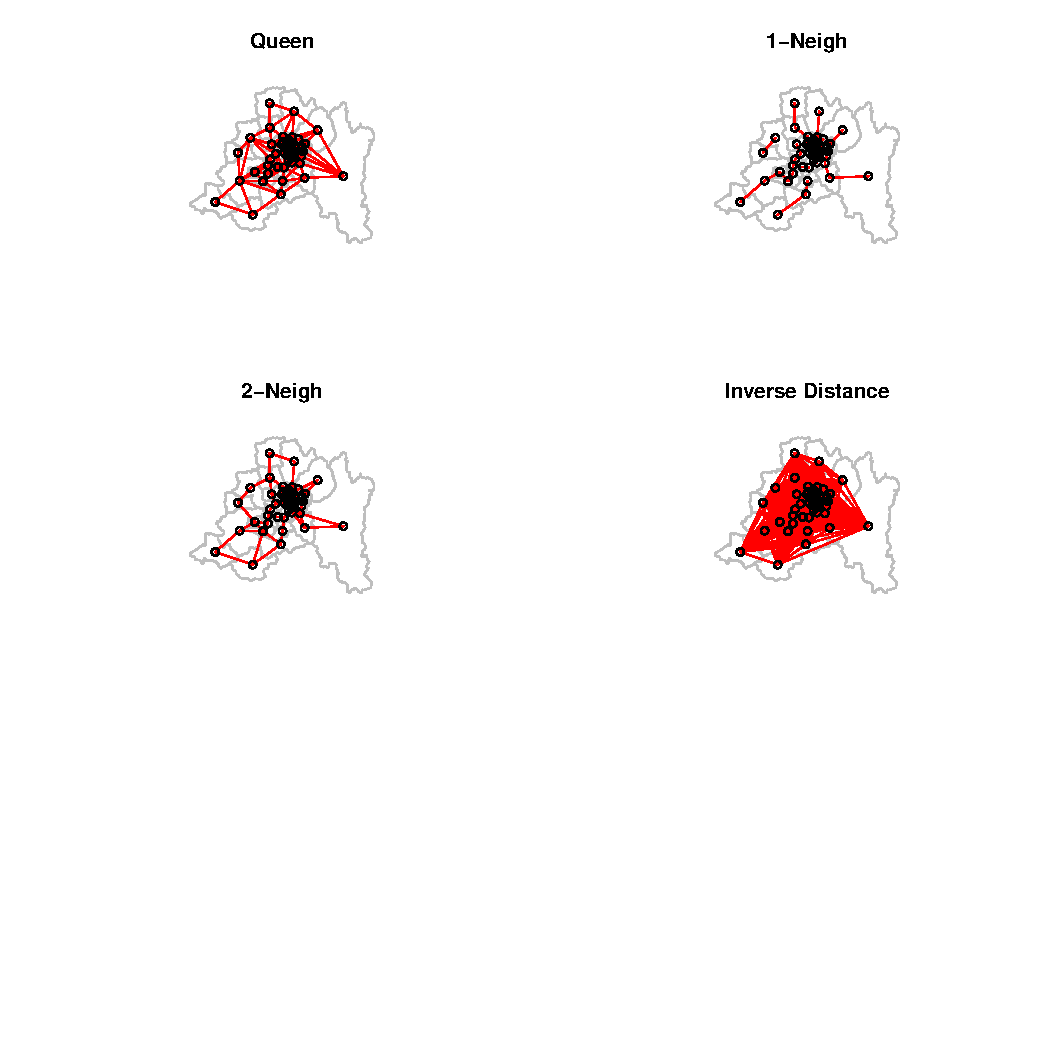
\includegraphics[width=\maxwidth]{figure/plot-all-wsT-1} 

}


\end{knitrout}
\end{figure}

\subsection{Constructing a Spatially Lagged Variable}

Spatially lagged variables are important elements of many spatial test and spatial regression specifications. In \pkg{spdep}, they are constructed by means of the \code{lag.listw} function.

First, we will combine the variables \code{POVERTY} and \code{URB\_POP} into a matrix and check the contents with \code{head}

\begin{knitrout}
\definecolor{shadecolor}{rgb}{0.969, 0.969, 0.969}\color{fgcolor}\begin{kframe}
\begin{alltt}
\hlcom{# X matrix}
\hlstd{X} \hlkwb{<-} \hlkwd{cbind}\hlstd{(mr}\hlopt{$}\hlstd{POVERTY, mr}\hlopt{$}\hlstd{URB_POP)}
\hlkwd{head}\hlstd{(X,} \hlnum{5}\hlstd{)}
\end{alltt}
\begin{verbatim}
##      [,1]   [,2]
## [1,]    8 159919
## [2,]    9  65262
## [3,]   18 131850
## [4,]   12 104634
## [5,]   14 166514
\end{verbatim}
\end{kframe}
\end{knitrout}

Now, we can construct a spatially lagged version of this matrix, using the \code{queen.w} weights\index{Weight matrix!lag.listw function}:

\begin{knitrout}
\definecolor{shadecolor}{rgb}{0.969, 0.969, 0.969}\color{fgcolor}\begin{kframe}
\begin{alltt}
\hlcom{# Create WX}
\hlstd{WX} \hlkwb{<-} \hlkwd{lag.listw}\hlstd{(}\hlkwd{nb2listw}\hlstd{(queen.w), X)}
\hlkwd{head}\hlstd{(WX)}
\end{alltt}
\begin{verbatim}
##          [,1]     [,2]
## [1,]  9.10000 100138.9
## [2,] 12.40000 299498.4
## [3,] 14.00000 144756.5
## [4,] 14.60000 121974.2
## [5,] 18.25000 170266.5
## [6,] 10.42857 236231.1
\end{verbatim}
\end{kframe}
\end{knitrout}


%****************************************************
\section{Testing for Spatial Autocorrelation}
%*****************************************************

As we stated in Section \ref{sec:Spatial_autocorrelation}, spatial autocorrelation refers to the correlation of a variable with itself in space. It can be positive (when high values correlate with high neighboring values or when low values correlate with low neighboring values) or negative (spatial outlier for high-low or low-high values). So the next question is how to test whether the spatial pattern we observe truly follows a spatial autocorrelated process or is completely random. In other words, we need a test of spatial autocorrelation to formally examine whether the observed value of a variable at one location is independent of values of that variable at neighboring locations.

%=============================================================
\subsection{Global Spatial Autocorrelation: Moran's I}\label{sec:moransI}
%============================================================

Global spatial autocorrelation is a measure of overall clustering. So the main goal of these indices is to summarize the degree to which similar observations tend to occur near each other. Those indices calculate the similarity of values at location $i$ and $j$ then `weight' the similarity by the proximity of locations $i$ and $j$. High similarities with high weight indicate similar values that are close together, whereas low similarities with high weight indicate dissimilar values that are close together.

The most general measure used is the Moran's I.\footnote{There exists several other measures of global spatial autocorrelation as the Geary's $C$ test. But, in this notes we will focus only in the Moran's I.} This statistic is a measure of overall clustering that exists in a dataset. It is assessed by means of a test of a null hypothesis of random location. Therefore, rejection of this null hypothesis suggests a spatial pattern or spatial structure. 

Moran's I is given by\index{Moran's I test}:

\begin{equation}\label{eq:I-moran}
I = \frac{\sum_{i = 1}^n\sum_{j=1, j\neq i}^n w_{ij}\left(x_i - \bar{x}\right)\left(x_j - \bar{x}\right)}{S_0 \sum_{i = 1}^n\left(x_i - \bar{x}\right)^2/n} = \frac{n\sum_{i = 1}^n\sum_{j=1}^n w_{ij}\left(x_i - \bar{x}\right)\left(x_j - \bar{x}\right)}{S_0 \sum_{i = 1}^n\left(x_i - \bar{x}\right)^2},
\end{equation}
%
where $S_0=\sum_{i = 1}^n\sum_{j=1}^nw_{ij}$ and $w_{ij}$ is an element of the spatial weight matrix that measures spatial distance or connectivity between regions $i$ and $j$. In matrix form:

\begin{equation*}
	I = \frac{n}{S_0} \frac{\vz^\top\mW\vz}{\vz^\top\vz},
\end{equation*}
%
where: 

\begin{equation*}
\vz = \begin{pmatrix}
          x_1 - \bar{x}\\
          x_2 - \bar{x} \\
          \vdots\\
          x_n - \bar{x}
      \end{pmatrix},
\end{equation*}

If the $\mW$ matrix is row standardized, then:

\begin{equation*}
	I = \frac{\vz^\top\mW^s\vz}{\vz^\top\vz},
\end{equation*}
%
because $S_0=n$. Values range from -1 (perfect dispersion) to +1 (perfect correlation). A zero value indicates a random spatial pattern. 

A very useful tool for understanding the Moran’s I test is the Moran Scatterplot. The idea of the Moran scatterplot is to display the variable for each region (on the horizontal axis) against the standardized spatial weighted average (average of the neighbors' $x$, also called spatial lag) on the vertical axis (See Figure \ref{fig:moran_scatterplot}). As pointed out by \cite{anselin1996chapter}, expressing the variables in standardized from (i.e. with mean zero and standard deviation equal to one) allows assessment of both the global spatial association, since the slope of the line is the Moran's I coefficient, and local spatial association (the quadrant in the scatterplot). The Moran scatterplot is therefore divided into four different quadrants corresponding to the four types of local spatial association between a region and its neighbors\index{Moran's I test!Moran scatterplot}:

\begin{itemize}
  \item Quadrant I displays the region with high $x$ (above the average) surrounded by regions with high $x$ (above the average). This quadrant is usually  denoted High-High.
  \item Quadrant II show the regions with low value surrounded by region with high values. This quadrant is usually denoted Low-High.
  \item Quadrant III display the regions with low value surrounded by regions with low values, and is denoted Low-Low.
  \item Quadrant IV shows the regions with high value surrounded by regions with low values. It is noted High-Low.
\end{itemize}

Regions located in quadrant I and III refer to positive spatial autocorrelation, the spatial clustering of similar values, whereas quadrant II and IV represent negative spatial autocorrelation, the spatial clustering of dissimilar values. 

\begin{figure}[ht]
  \caption{Moran Scatterplot}\label{fig:moran_scatterplot}
\begin{knitrout}
\definecolor{shadecolor}{rgb}{0.969, 0.969, 0.969}\color{fgcolor}

{\centering 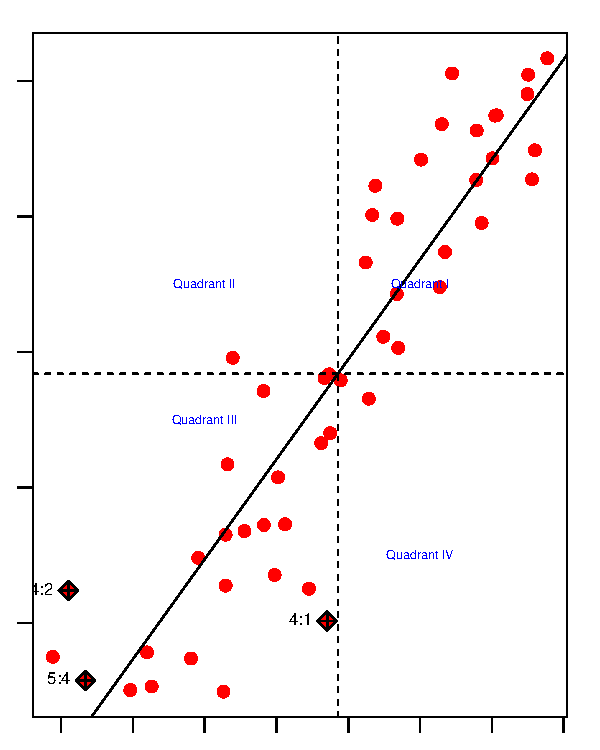
\includegraphics[width=\maxwidth]{figure/moran-1} 

}


\end{knitrout}
\end{figure}


To understand Moran's I, it is important to note the similarity of the Moran's $I$ with the OLS coefficient. Recall that 

\begin{equation}
  \widehat{\vbeta}= \frac{\sum_{i = 1}^n\left(x_i - \bar{x}\right)(y_i - \bar{y})}{\sum_{i = 1}^n \left(x_i - \bar{x}\right)^2}
\end{equation}

Then looking at (\ref{eq:I-moran}), Moran's $I$ is equivalent to the slope coefficient of a linear regression of the spatial lag $\mW\vx$ on the observation vector $\vx$ measured in deviation from their mean. It is, however, not equivalent to the slope of $\vx$ on $\mW\vx$ which would be a more natural way. 

The hypothesis tested by the Moran's $I$ is the following:

\begin{itemize}
  \item $H_0$: $\vx$ is spatially independent; the observed $\vx$ is assigned at random among locations. In this case $I$ is close to zero.
  \item $H_1$: $\vx$ is not spatially independent. In this case $I$ is statistically different from zero. 
\end{itemize}

What is the distribution of the Moran's I? We are interested in the distribution of:

\begin{equation*}
  \frac{I - \E\left[I\right]}{\sqrt{\var(I)}}
\end{equation*}

There are two ways to compute the mean and variance of Moran's I. The first one is under the normal assumption of $x_i$ and the second one is under randomization of $x_i$. Under the normal assumption, it is assumed that the random variable $x_i$ are the result of $n$ independently drawings from a normal population. Under the randomization assumption, no matter what the underlying distribution of the populations, we consider the observed values of $x_i$ were repeatedly randomly permuted.

\subsubsection{Moments Under Normality Assumption}

Theorem \ref{teo:Moran_normal} gives the moments of Moran's I under normality. 

\begin{theorem}[Moran's $I$ Under Normality]\label{teo:Moran_normal}\index{Moran's I test!Normality}
Assume that $\left\lbrace \vx_i\right\rbrace = \left\lbrace x_1, x_2,..., x_n\right\rbrace$ are independent and distributed as $\rN(\mu, \sigma^2)$, but $\mu$ and $\sigma^2$ are unknown. Then:

\begin{equation}
\E\left(I\right) = - \frac{1}{n - 1} 
\end{equation}
%
and

\begin{equation}
\E\left(I^2\right) = \frac{n^2S_1 - nS_2 + 3S_0^2}{S_0^2(n^2 - 1)}
\end{equation}
%
where $S_0=\sum_{i = 1}^n\sum_{j=1}^nw_{ij}$, $S_1= \sum_{i = 1}^n\sum_{j = 1}^n(w_{ij} + w_{ji})^2/2$, $S_2 = \sum_{i = 1}^n(w_{i.} + w_{.i})^2$, where $w_{i.}= \sum_{j = 1}^nw_{ij}$ and $w_{i.}=\sum_{j = 1}^nw_{ji}$
Then:

\begin{equation}
\var\left(I\right)=\E\left(I^2\right) - \E\left(I\right)^2
\end{equation}
\end{theorem}

\begin{proof}
Let $z_i=x_i - \bar{x}$. The following moments are true for $z_i$:

\begin{eqnarray*}
\E\left[z_i\right]   & = & 0 \\
\E\left[z_i^2\right] & = & \sigma^2 - \frac{\sigma^2}{n} \\
\E\left[z_iz_j\right] & = & - \frac{\sigma^2}{n} \\
\E\left[z_i^2 z_j^2\right] & = & \frac{(n^2 - 2n + 3)\sigma^2}{m^2} \\
\E\left[z_i^2 z_jz_k\right] & = & - \frac{(n -3)\sigma^4}{n} \\
\E\left[z_iz_jz_kz_l\right] & = & \frac{3 \sigma^4}{n^2}
\end{eqnarray*}


Then:

\begin{equation}
  \begin{aligned}
    \E\left[I\right] & = \frac{n}{S_0}\frac{\E\left[\sum_{i = 1}^n\sum_{j=1}^nw_{ij}z_iz_j\right]}{\E\left[\sum_{i=1}^nz_i^2\right]}
    & = \frac{n}{S_0}\sum_{i = 1}^n\sum_{j=1}^nw_{ij}\frac{\E\left[z_iz_j\right]}{\sum_{i=1}^n\E\left[z_i^2\right]} \\
    & = \frac{-nS_0\frac{\sigma^2}{n}}{S_0 n (1 - 1/n)\sigma^2 } \\
    & = -\frac{\frac{\sigma^2}{n}}{(1 - 1/n)\sigma^2 } \\
    & = -\frac{1}{n - 1} 
  \end{aligned}
\end{equation}

and

\begin{equation}
  \begin{aligned}
    \E\left[I^2\right] & = \E\left[\frac{n^2}{S_0^2}\frac{\left[\sum_{i = 1}^n\sum_{j=1}^nw_{ij}z_iz_j\right]^2}{\left[\sum_{i=1}^nz_i^2\right]^2}\right] \\
    & = \frac{n^2}{S_0^2} \E\left[\frac{1/2\sum_{(2)}(w_{ij} + w_{ji})^2 z_i^2 z_j^2 + \sum_{(3)}(w_{ij} + w_{ji})(w_{ik} + w_{ki})z_i^2z_jz_k + \sum_{(4)} w_{ij}w_{kl}z_iz_jz_kz_l}{s}\right]
  \end{aligned}
\end{equation}
\end{proof}

\subsubsection{Moran's $I$ under Randomization}

%Recall that when testing a null hypothesis we need a test statistic that will have different values under the null hypothesis and the alternatives. We then need to compute the sampling distribution of the test statistic when the null hypothesis is true. For some test statistics and some null hypotheses this can be done analytically. Then, the $p$-value is the probability that the test statistic would be at least as extreme as we observed, if the null hypothesis is true.

%A permutation test gives a simple way to compute the sampling distribution for any test statistic. 

%To estimate the sampling distribution of the test statistic we need many samples generated under the strong null hypothesis. A permutation test builds sampling distribution by resampling the observed data. Specifically, we can ``shuffle'' or permute the observed data by 


%A randomization test (also called a permutation test) is a type of statistical significance test in which the distribution of the test statistic under the null hypothesis is obtained by calculating all possible values of the test statistics under rearrangements of the labels on the observed points. 

%No matter what the underlying distribution of the population, we consider the observed values of $x_i$ were repeatedly randomly permuted.


%Under randomization 

%The testing method under randomization assumption is called permutation test. 

Theorem \ref{teo:Moran_random} gives the moments of Moran's I under randomization. 


\begin{theorem}[Moran's $I$ Under Randomization]\label{teo:Moran_random}\index{Moran's I test!Randomization}
Under permutation, we have:

\begin{equation}
\E\left(I\right) = - \frac{1}{n - 1} 
\end{equation}
%
and

\begin{equation}
\E\left(I^2\right) = \frac{n\left[\left(n^2 - 3n + 3\right)S_1 - nS_2 + 3S_0^2\right]-b_2\left[\left(n^2 - n\right)S_1 - 2nS_2 + 6S_0^2\right]}{(n-1)(n-2)(n-3)S_0^2}
\end{equation}
%
where $S_0=\sum_{i = 1}^n\sum_{j=1}^nw_{ij}$, $S_1= \sum_{i = 1}^n\sum_{j = 1}^n(w_{ij} + w_{ji})^2/2$, $S_2 = \sum_{i = 1}^n(w_{i.} + w_{.i})^2$, where $w_{i.}= \sum_{j = 1}^nw_{ij}$ and $w_{i.}=\sum_{j = 1}^nw_{ji}$.Then:

\begin{equation}
\var\left(I\right)=\E\left(I^2\right) - \E\left(I\right)^2
\end{equation}
\end{theorem}

It is important to note that the expected value of Moran's $I$ under normality and randomization is the same. 

\subsubsection{Monte Carlo Moran's $I$}

The normality assumption is a very strong assumption. However we can use the Moran’s I test based on Monte Carlo simulation.

The idea for any Monte Carlo test is the following\index{Moran's I test!Monte carlo}: 

\begin{itemize}
  \item To test a null hypothesis $H_0$ (no spatial autocorrelation in our case), we specify a test statistic $T$ such that large values of $T$ are evidence against $H_0$.
  \item Let $T$ have observed value $t_{obs}$. We generally want to compute
  
  \begin{equation}
    p-value = \Pr(T\geq t_{obs}|H_0)
  \end{equation}
  
  Therefore we need the distribution of $T$ when $H_0$ is true to evaluate this probability.
\end{itemize}

The algorithm for the Morans' I Monte Carlo test is the following:

\begin{algorithm}[Moran's' I Monte Carlo Test]
The procedure is the following:

\begin{enumerate}
\item Rearrange the spatial data by shuffling their location and compute the Moran's I $S$ times. This will create the distribution under $H_0$. This operationalizes spatial randomness. 
\item Let $I_1^*, I_2^*,..., I_S^*$ be the Moran's I for each time. A consistent Monte Carlo p-value is then:
  \begin{equation}
    \widehat{p} = \frac{1 + \sum_{s=1}^S 1(I^*_s \geq I_{obs})}{S + 1}
  \end{equation}
  \item For tests at the $\alpha$ level or at $100(1- \alpha)\%$ confidence intervals, there are reasons for choosing $S$ so that $\alpha(S + 1)$ is an integer. For example, use $S=999$ for confidence intervals and hypothesis tests when $\alpha = 0.05$.
\end{enumerate}
\end{algorithm}


%%=====================================================
%\subsection{Local Indicators of Spatial Association (LISA)}
%=====================================================

%\cite{anselin1995local} suggests that a local indicator of spatial association (LISA) is any statistic that satisfies the following two requirements:

%\begin{enumerate}
%  \item the LISA for each observation gives an indication of the extent of significant spatial clustering of similar values around that observation;
%  \item the sum of LISAs for all observations is proportional to a global indicator of spatial association.
%\end{enumerate}

%=====================================================
\section{Application: Poverty in Santiago, Chile}
%=====================================================

In this section we undertake and exploratory spatial data analysis (ESDA) for poverty in Metropolitan Region, Chile.  


%================================
\subsection{Cloropeth Graphs}
%================================

If we are interested in the geographical variation in poverty, we should start by plotting the spatial distribution of poverty.  This can be useful in a variety of way.  Usually, aggregate or national level indicators hide important differences between different spatial units. Thus, poverty mapping helps to highlight geographical variations.  In addition to this, another advantage of poverty maps is their legibility- maps are powerful tools for representing complex information in a visual format that is easy to understand. 

So, we start by plotting the geographical variation of poverty among communes by using the \code{plot} function. In particular, we use a cloropleth\footnote{The name of this technique is derived from the Greek words choros - space, and pleth - value} map using the quantile classification. In a quantile graph, the variable is sorted and grouped in categories with equal number of observations, or quantiles. 


\begin{knitrout}
\definecolor{shadecolor}{rgb}{0.969, 0.969, 0.969}\color{fgcolor}\begin{kframe}
\begin{alltt}
\hlcom{# Cloropleth graphs ----}
\hlkwd{library}\hlstd{(}\hlstr{"RColorBrewer"}\hlstd{)}
\hlkwd{plot}\hlstd{(mr[}\hlstr{"POVERTY"}\hlstd{],}
       \hlkwc{breaks} \hlstd{=} \hlstr{"quantile"}\hlstd{,}
       \hlkwc{nbreaks} \hlstd{=} \hlnum{5}\hlstd{,}
       \hlkwc{pal} \hlstd{=} \hlkwd{brewer.pal}\hlstd{(}\hlnum{5}\hlstd{,} \hlstr{"Blues"}\hlstd{),}
       \hlkwc{main} \hlstd{=} \hlstr{""}\hlstd{,}
       \hlkwc{axes} \hlstd{=} \hlnum{TRUE}\hlstd{)}
\end{alltt}
\end{kframe}
\end{knitrout}

Figure \ref{fig:cloro-graph} provides some useful insights. First, it clearly shows that the spatial pattern of poverty in the MR is not spatial homogeneous, but rather the intensity of poverty varies across space. Second, it provides an example of how disaggregated poverty indicators can reveal additional information to aggregate indicators. It shows that poverty intensity is lower peripheral communes than central communes. 

\begin{figure}
\caption{Cloropleth map: Poverty in the Metropolitan Region}\label{fig:cloro-graph}
\begin{knitrout}
\definecolor{shadecolor}{rgb}{0.969, 0.969, 0.969}\color{fgcolor}

{\centering 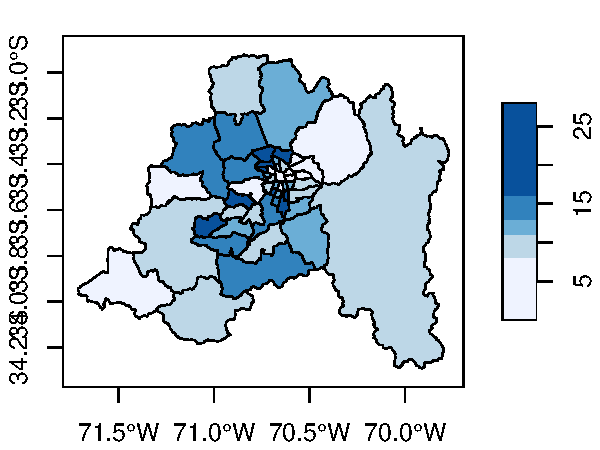
\includegraphics[width=\maxwidth]{figure/cloro-graphs-1} 

}


\end{knitrout}
\end{figure}

How to interpret quantile maps? A quantile classification scheme is an ordinal ranking of the data values, dividing the distribution into intervals that have an equal number of data values. Quantile classification ensures maps are easily comparable and can be `easy to read'.

% We can also plot the data using the equal interval classification. Equal interval divides the data into equal size classes (e.g., 0-10, 10-20, 20-30, etc) and works best on data that is generally spread across the entire range. In the following example we use a defined interval classification. 
% 
% <<cloro-graphs2F, eval =  FALSE>>=
% # Define interval classification 
% mr$pov.cat <- cut(mr$POVERTY, 
%                   breaks = c(0, 9, 12, 16, 28),
%                   labels = c("< 9", "9-12", "12-16", ">16"))
% spplot(mr, "pov.cat", col.regions = brewer.pal(5, "Reds"))
% @
% 
% \begin{figure}[h]
% \caption{Cloropleth map: Poverty in the Metropolitan Region (Equal Interval)}\label{fig:cloro-graph2}
% <<cloro-graphs2T, fig.align='center', fig.height = 3, fig.width = 4, fig.show='hold', echo = FALSE>>=
% plot(mr["POVERTY"], 
%        breaks = "quantile",
%        nbreaks = 5, 
%        pal = brewer.pal(5, "Blues"), 
%        main = "", 
%        axes = TRUE)
% @
% \end{figure}


However, regarding the possible spatial association that seems to be derived from the above figure for the poverty variable, it is necessary to note that the results are sensitive to the number of defined intervals (among other things). Therefore, it is necessary to conduct a comprehensive and formal analysis about the potential presence of spatial dependence to ascertain whether there exists a pattern of statistically significant spatial autocorrelation in the spatial distribution of poverty. That is why now we calculate the Moran’s I test.


%================================
\subsection{Moran's I Test}
%================================

First, we create two spatial weight matrices (queen and rook) to assess the robustness of the test under different spatial schemes. 

\begin{knitrout}
\definecolor{shadecolor}{rgb}{0.969, 0.969, 0.969}\color{fgcolor}\begin{kframe}
\begin{alltt}
\hlcom{# Generate W matrices}
\hlstd{queen.w} \hlkwb{<-} \hlkwd{poly2nb}\hlstd{(}\hlkwd{as}\hlstd{(mr,} \hlstr{"Spatial"}\hlstd{),} \hlkwc{row.names} \hlstd{= mr}\hlopt{$}\hlstd{NAME,} \hlkwc{queen} \hlstd{=}  \hlnum{TRUE}\hlstd{)}
\hlstd{rook.w}  \hlkwb{<-} \hlkwd{poly2nb}\hlstd{(}\hlkwd{as}\hlstd{(mr,} \hlstr{"Spatial"}\hlstd{),} \hlkwc{row.names} \hlstd{= mr}\hlopt{$}\hlstd{NAME,} \hlkwc{queen} \hlstd{=}  \hlnum{FALSE}\hlstd{)}
\end{alltt}
\end{kframe}
\end{knitrout}

Moran's I test statistic for spatial autocorrelation is implemented in \pkg{spdep} \citep{spdep}. There are mainly two function for computing this test: \code{moran.test}, where the inference is based on a normal or randomization assumption, and \code{moran.mc}, for a permutation-based test\index{Moran's I test!moran.test function}. 

\begin{knitrout}
\definecolor{shadecolor}{rgb}{0.969, 0.969, 0.969}\color{fgcolor}\begin{kframe}
\begin{alltt}
\hlcom{# Moran's I test}
\hlkwd{moran.test}\hlstd{(mr}\hlopt{$}\hlstd{POVERTY,} \hlkwc{listw} \hlstd{=} \hlkwd{nb2listw}\hlstd{(queen.w),} \hlkwc{randomisation} \hlstd{=} \hlnum{FALSE}\hlstd{,}
           \hlkwc{alternative} \hlstd{=} \hlstr{'two.sided'}\hlstd{)}
\end{alltt}
\begin{verbatim}
## 
## 	Moran I test under normality
## 
## data:  mr$POVERTY  
## weights: nb2listw(queen.w)    
## 
## Moran I statistic standard deviate = 4.0453, p-value = 5.225e-05
## alternative hypothesis: two.sided
## sample estimates:
## Moran I statistic       Expectation          Variance 
##       0.306497992      -0.019607843       0.006498517
\end{verbatim}
\begin{alltt}
\hlkwd{moran.test}\hlstd{(mr}\hlopt{$}\hlstd{POVERTY,} \hlkwc{listw} \hlstd{=} \hlkwd{nb2listw}\hlstd{(rook.w),} \hlkwc{randomisation} \hlstd{=} \hlnum{FALSE}\hlstd{,}
           \hlkwc{alternative} \hlstd{=} \hlstr{'two.sided'}\hlstd{)}
\end{alltt}
\begin{verbatim}
## 
## 	Moran I test under normality
## 
## data:  mr$POVERTY  
## weights: nb2listw(rook.w)    
## 
## Moran I statistic standard deviate = 4.3309, p-value = 1.485e-05
## alternative hypothesis: two.sided
## sample estimates:
## Moran I statistic       Expectation          Variance 
##       0.342282943      -0.019607843       0.006982432
\end{verbatim}
\end{kframe}
\end{knitrout}

The \code{randomisation} option is set to \code{TRUE} by default, which implies that in order to get inference based on a normal approximation, it must be explicitly set to \code{FALSE}, as in our case. Similarly, the default is a one-sided test, so that in order to obtain the results for the more commonly used two-sided test, the option \code{alternative} must be explicitly to \code{'two.sided'}. Note also that the \code{zero.policy} option is set to \code{FALSE} by default, which means that islands result in a missing value code \code{NA}. Setting this option to \code{TRUE} will set the spatial lag for island to the customary zero value. 

The results show that the Moran's I statistic are $\approx$ 0.30 and 0.34, respectively, and highly significant. This implies that there is evidence of robust \textbf{positive spatial autocorrelation} in the poverty variable (since we are rejecting the null hypothesis of random spatial distribution).


\begin{remark}
If you compute the Moran's I test for two different variables, but using the same spatial weight matrix, the expectation and variance of the Moran's I test statistic will be the same under the normal approximation. Why? 
\end{remark}

The test under randomization gives the following results:

\begin{knitrout}
\definecolor{shadecolor}{rgb}{0.969, 0.969, 0.969}\color{fgcolor}\begin{kframe}
\begin{alltt}
\hlcom{# Moran test under randomization}
\hlkwd{moran.test}\hlstd{(mr}\hlopt{$}\hlstd{POVERTY,} \hlkwc{listw} \hlstd{=} \hlkwd{nb2listw}\hlstd{(queen.w),}
           \hlkwc{alternative} \hlstd{=} \hlstr{'two.sided'}\hlstd{)}
\end{alltt}
\begin{verbatim}
## 
## 	Moran I test under randomisation
## 
## data:  mr$POVERTY  
## weights: nb2listw(queen.w)    
## 
## Moran I statistic standard deviate = 4.0689, p-value = 4.723e-05
## alternative hypothesis: two.sided
## sample estimates:
## Moran I statistic       Expectation          Variance 
##       0.306497992      -0.019607843       0.006423226
\end{verbatim}
\end{kframe}
\end{knitrout}

Note how the value of the statistic and its expectation do not change relative to the normal case, only the variance is different.

We can carry out a Moran's $I$ test based on random permutation the function \code{moran.mc}. Unlike previous test, it needs the number of permutations \code{nsim}. Since the rank of the observed statistic is computed relative to the reference distribution of statistics for the permuted data sets, it is good practice to set this number to something ending on 9 (such as 99 or 999). This will lead to rounded pseudo p-values like 0.01 or 0.001.\index{Moran's I test!moran.mc function} 


\begin{knitrout}
\definecolor{shadecolor}{rgb}{0.969, 0.969, 0.969}\color{fgcolor}\begin{kframe}
\begin{alltt}
\hlcom{# Moran's Test}
\hlkwd{set.seed}\hlstd{(}\hlnum{1234}\hlstd{)}
\hlkwd{moran.mc}\hlstd{(mr}\hlopt{$}\hlstd{POVERTY,} \hlkwc{listw} \hlstd{=} \hlkwd{nb2listw}\hlstd{(queen.w),}
           \hlkwc{nsim} \hlstd{=} \hlnum{99}\hlstd{)}
\end{alltt}
\begin{verbatim}
## 
## 	Monte-Carlo simulation of Moran I
## 
## data:  mr$POVERTY 
## weights: nb2listw(queen.w)  
## number of simulations + 1: 100 
## 
## statistic = 0.3065, observed rank = 100, p-value = 0.01
## alternative hypothesis: greater
\end{verbatim}
\end{kframe}
\end{knitrout}


Note that none of the permuted data sets yielded a Moran's $I$ greater than the observed value of 0.3065, hence a pseudo p-value of $(0 + 1) / (99 + 1) = 0.01$.

The Moran scatter plot can also be obtained using the function \code{moran.plot} of \pkg{spdep}:\index{Moran's I test!moran.plot function}

\begin{knitrout}
\definecolor{shadecolor}{rgb}{0.969, 0.969, 0.969}\color{fgcolor}\begin{kframe}
\begin{alltt}
\hlcom{# Moran's plot}
\hlkwd{moran.plot}\hlstd{(mr}\hlopt{$}\hlstd{POVERTY,} \hlkwc{listw} \hlstd{=} \hlkwd{nb2listw}\hlstd{(queen.w))}
\end{alltt}
\end{kframe}
\end{knitrout}

\begin{figure}[ht]
\caption{Moran Plot for Poverty}\label{fig:mp-poverty}
\begin{knitrout}
\definecolor{shadecolor}{rgb}{0.969, 0.969, 0.969}\color{fgcolor}

{\centering 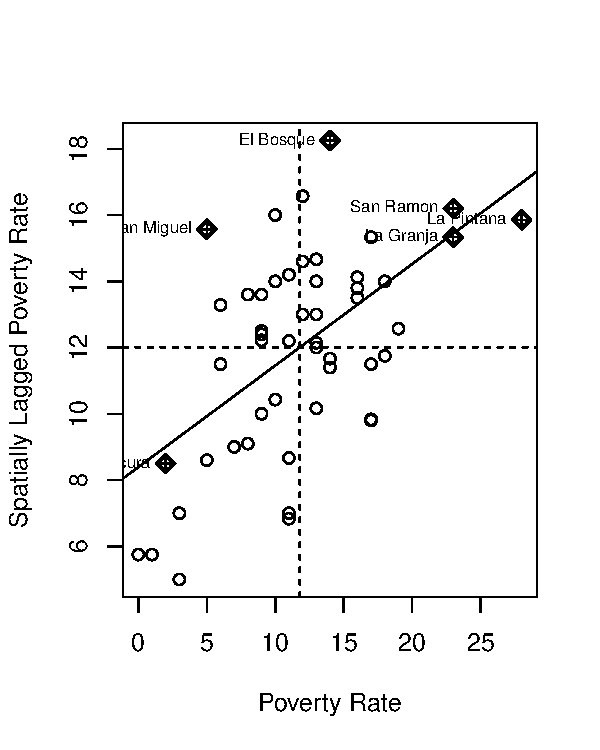
\includegraphics[width=\maxwidth]{figure/moran-plotT-1} 

}


\end{knitrout}
\end{figure}

Figure \ref{fig:mp-poverty} displays the Moran scatterplot of poverty with the queen weight matrix. Positive spatial autocorrelation, detected by the value of the Moran's I, is reflected by the fact that most of the communes are located in quadrant I and III. However, there are some exceptions such as the communes located in quadrant II and IV. For example, San Miguel is a commune with low poverty rate, but surrounded by communes with high poverty.  

A major limitation of Moran's I is that it cannot provide information on the specific locations of spatial patterns; it only indicates the presence of spatial autocorrelation globally. A single overall indication is given of whether spatial autocorrelation exists in the dataset, but no indication is given of whether local variations exist in spatial autocorrelation (e.g., concentrations, outliers) across the spatial extent of the data. 


%-----------------------
\section{Exercises}
%-------------------

\begin{exercises}
 \exercise Another method used for creating spatial weight matrices in Monte Carlo studies is the ``$k$-ahead and $k$-behind'' criterion in a circular world. (This was introduced by \cite{kelejian1999generalized}). In this approach, each spatial unit is assumed to have $k$ neighbors which are ahead of it in the order of sample, and $k$ units which are behind it. The number $k$ is typically chosen to be small relative to the sample size. Thus, each spatial unit has $2k$ neighbors. Weighting matrices which are built on this framework are typically row normalized, and all of the nonzero elements in the matrix are $1/(2k)$. Suppose $n =10$ and $k =2$. Specify the third row of the $10\times 10$ weighting matrix.
 \exercise For a general sample size, say $n$, which corresponds to a checkerboard of squares, what is the minimum number of neighbors a unit can have if the weighting matrix is based on a queen pattern?
 \exercise  Let $INC_r$ the income per capita in cross-sectional unit $r = 1, ...., n$. Consider the following specification for $w_{ij}$:
	
	\begin{equation*}
	w_{ij}= \alpha\left[1 - \frac{\left|INC_i - INC_j\right|}{INC_i+ INC_j}\right], 
	\end{equation*}
	%
	where $\alpha$ is some pre-selected positive constant. Show that $\alpha$ will cancel if the weight matrix is row-normalized.
	\exercise  Create in \proglang{R} your own function to plot a Moran Scatterplot. Show that your function works well using a simulated example. 
\end{exercises}
